\documentclass[twoside]{book}

% Packages required by doxygen
\usepackage{fixltx2e}
\usepackage{calc}
\usepackage{doxygen}
\usepackage[export]{adjustbox} % also loads graphicx
\usepackage{graphicx}
\usepackage[utf8]{inputenc}
\usepackage{makeidx}
\usepackage{multicol}
\usepackage{multirow}
\PassOptionsToPackage{warn}{textcomp}
\usepackage{textcomp}
\usepackage[nointegrals]{wasysym}
\usepackage[table]{xcolor}

% Font selection
\usepackage[T1]{fontenc}
\usepackage[scaled=.90]{helvet}
\usepackage{courier}
\usepackage{amssymb}
\usepackage{sectsty}
\renewcommand{\familydefault}{\sfdefault}
\allsectionsfont{%
  \fontseries{bc}\selectfont%
  \color{darkgray}%
}
\renewcommand{\DoxyLabelFont}{%
  \fontseries{bc}\selectfont%
  \color{darkgray}%
}
\newcommand{\+}{\discretionary{\mbox{\scriptsize$\hookleftarrow$}}{}{}}

% Page & text layout
\usepackage{geometry}
\geometry{%
  a4paper,%
  top=2.5cm,%
  bottom=2.5cm,%
  left=2.5cm,%
  right=2.5cm%
}
\tolerance=750
\hfuzz=15pt
\hbadness=750
\setlength{\emergencystretch}{15pt}
\setlength{\parindent}{0cm}
\setlength{\parskip}{3ex plus 2ex minus 2ex}
\makeatletter
\renewcommand{\paragraph}{%
  \@startsection{paragraph}{4}{0ex}{-1.0ex}{1.0ex}{%
    \normalfont\normalsize\bfseries\SS@parafont%
  }%
}
\renewcommand{\subparagraph}{%
  \@startsection{subparagraph}{5}{0ex}{-1.0ex}{1.0ex}{%
    \normalfont\normalsize\bfseries\SS@subparafont%
  }%
}
\makeatother

% Headers & footers
\usepackage{fancyhdr}
\pagestyle{fancyplain}
\fancyhead[LE]{\fancyplain{}{\bfseries\thepage}}
\fancyhead[CE]{\fancyplain{}{}}
\fancyhead[RE]{\fancyplain{}{\bfseries\leftmark}}
\fancyhead[LO]{\fancyplain{}{\bfseries\rightmark}}
\fancyhead[CO]{\fancyplain{}{}}
\fancyhead[RO]{\fancyplain{}{\bfseries\thepage}}
\fancyfoot[LE]{\fancyplain{}{}}
\fancyfoot[CE]{\fancyplain{}{}}
\fancyfoot[RE]{\fancyplain{}{\bfseries\scriptsize Generated by Doxygen }}
\fancyfoot[LO]{\fancyplain{}{\bfseries\scriptsize Generated by Doxygen }}
\fancyfoot[CO]{\fancyplain{}{}}
\fancyfoot[RO]{\fancyplain{}{}}
\renewcommand{\footrulewidth}{0.4pt}
\renewcommand{\chaptermark}[1]{%
  \markboth{#1}{}%
}
\renewcommand{\sectionmark}[1]{%
  \markright{\thesection\ #1}%
}

% Indices & bibliography
\usepackage{natbib}
\usepackage[titles]{tocloft}
\setcounter{tocdepth}{3}
\setcounter{secnumdepth}{5}
\makeindex

% Hyperlinks (required, but should be loaded last)
\usepackage{ifpdf}
\ifpdf
  \usepackage[pdftex,pagebackref=true]{hyperref}
\else
  \usepackage[ps2pdf,pagebackref=true]{hyperref}
\fi
\hypersetup{%
  colorlinks=true,%
  linkcolor=blue,%
  citecolor=blue,%
  unicode%
}

% Custom commands
\newcommand{\clearemptydoublepage}{%
  \newpage{\pagestyle{empty}\cleardoublepage}%
}

\usepackage{caption}
\captionsetup{labelsep=space,justification=centering,font={bf},singlelinecheck=off,skip=4pt,position=top}

%===== C O N T E N T S =====

\begin{document}

% Titlepage & ToC
\hypersetup{pageanchor=false,
             bookmarksnumbered=true,
             pdfencoding=unicode
            }
\pagenumbering{alph}
\begin{titlepage}
\vspace*{7cm}
\begin{center}%
{\Large Learn with Robin }\\
\vspace*{1cm}
{\large Generated by Doxygen 1.8.13}\\
\end{center}
\end{titlepage}
\clearemptydoublepage
\pagenumbering{roman}
\tableofcontents
\clearemptydoublepage
\pagenumbering{arabic}
\hypersetup{pageanchor=true}

%--- Begin generated contents ---
\chapter{R\+E\+A\+D\+ME}
\label{md__c_1__users__jean-_loup__documents__l3__projet_malette_jeux__q_t__l_w_robin__learn_with_robin_main__r_e_a_d_m_e}
\Hypertarget{md__c_1__users__jean-_loup__documents__l3__projet_malette_jeux__q_t__l_w_robin__learn_with_robin_main__r_e_a_d_m_e}
Learn\+With\+Robin\+Main 
\chapter{Test List}
\label{test}
\Hypertarget{test}

\begin{DoxyRefList}
\item[\label{test__test000002}%
\Hypertarget{test__test000002}%
Member \hyperlink{class_main_menu_acacb97bab2a77bd09dedccea22a32116}{Main\+Menu\+:\+:go\+For\+Puzzle} (void)]pour l\textquotesingle{}instant sert à tester la sauvegarde  
\item[\label{test__test000001}%
\Hypertarget{test__test000001}%
Member \hyperlink{class_main_menu_a891bed1e0edb5492671c332cb89b7a9a}{Main\+Menu\+:\+:Main\+Menu} (Q\+Widget $\ast$parent=nullptr)]nouvelle syntaxe connexion signal slot  
\item[\label{test__test000004}%
\Hypertarget{test__test000004}%
Member \hyperlink{class_robin_main_window_a55f7775f5daefb2099a51e97d50df666}{Robin\+Main\+Window\+:\+:Robin\+Main\+Window} (Q\+Widget $\ast$parent=0)]changer la fenetre on peut tenter vu que Q\+Widget hérite de Q\+Object 

test très fort  
\item[\label{test__test000006}%
\Hypertarget{test__test000006}%
Member \hyperlink{class_super_simon_af12663f8a26a971a508a40a33d0afceb}{Super\+Simon\+:\+:delay} (int \&sec)]
\end{DoxyRefList}
\chapter{Todo List}
\label{todo}
\Hypertarget{todo}

\begin{DoxyRefList}
\item[\label{todo__todo000005}%
\Hypertarget{todo__todo000005}%
Member \hyperlink{class_memory_a7c8b57775899a3782edcdf4da430ad61}{Memory\+:\+:get\+Nb\+Cards} (void)]faire un modèle 

récupérer dans le modèle après  
\item[\label{todo__todo000001}%
\Hypertarget{todo__todo000001}%
Member \hyperlink{class_memory_a243eef3e0fd8d02131e3bcca0471c931}{Memory\+:\+:Memory} (Q\+Widget $\ast$parent=0)]ordonner / ranger un peu cette fonction 

faire en sorte de régler le nombre de cartes selon la difficulté 

gérer le nombre de lignes et colonnes par rapport au nombre de cartes par exemple avec une approche de la racine carrée par la valeur inférieure pour les lignes, puis continuer à remplir dans les cases en revenant à la ligne à chaque fin de ligne, jusqu\textquotesingle{}à l\textquotesingle{}écoulement des cartes  
\item[\label{todo__todo000004}%
\Hypertarget{todo__todo000004}%
Member \hyperlink{class_memory_ad9a06b40d30c5ee3bbccacb37795255b}{Memory\+:\+:paint\+Event} (Q\+Paint\+Event $\ast$)]vérifier ce que ça fait je pense que c\textquotesingle{}est pour stocker les rectangles dessinés dans le tableau mentionné ça sert peut-\/être à rien ici  
\item[\label{todo__todo000007}%
\Hypertarget{todo__todo000007}%
Class \hyperlink{class_memory_index_cards}{Memory\+Index\+Cards} ]il faudra un générateur de stylesheet efficace  
\item[\label{todo__todo000008}%
\Hypertarget{todo__todo000008}%
Member \hyperlink{class_memory_index_cards_a10ae71958cd423edde68dc41dd010a66}{Memory\+Index\+Cards\+:\+:Memory\+Index\+Cards} (std\+::string \&pathcsv)]implémenter  
\item[\label{todo__todo000011}%
\Hypertarget{todo__todo000011}%
Member \hyperlink{class_mod_calcul_aa16185334bb48c8e312bd0b9148aa00d}{Mod\+Calcul\+:\+:get\+Ope1\+Str} (void)]implémenter  
\item[\label{todo__todo000010}%
\Hypertarget{todo__todo000010}%
Member \hyperlink{class_mod_calcul_ad6061decce032f0debf6fa79d153df5d}{Mod\+Calcul\+:\+:ini\+Set\+Operateurs} (pos\+Set\+Op set\+Op)]gérer ça 

gérer ça  
\item[\label{todo__todo000014}%
\Hypertarget{todo__todo000014}%
Member \hyperlink{class_mod_memory_a4e6581fef7b3adbad429bf4c39d38e88}{Mod\+Memory\+:\+:close\+Cards} (void)]C\+O\+M\+P\+L\+E\+T\+ER en retournant les trucs de flipped card et verifier qu\textquotesingle{}on ne manipule pas flippedcard dans les methodes ou l\textquotesingle{}on devrait manipuler cards

arreter d\textquotesingle{}etre malade  
\item[\label{todo__todo000013}%
\Hypertarget{todo__todo000013}%
Member \hyperlink{class_mod_memory_a77d39288e861c84edcfa760170fbc44d}{Mod\+Memory\+:\+:$\sim$\+Mod\+Memory} ()]supprimer contenu des vecteurs et les vider  
\item[\label{todo__todo000019}%
\Hypertarget{todo__todo000019}%
Member \hyperlink{class_mod_simon_a01de269fc7beadbe1199c233ba24ada4}{Mod\+Simon\+:\+:ini\+Score\+To\+Reach} (void)]implémenter difficulté  
\item[\label{todo__todo000026}%
\Hypertarget{todo__todo000026}%
Member \hyperlink{class_robin_main_window_a0850e17ae24394b14eb2dcfc4f15eeca}{Robin\+Main\+Window\+:\+:back\+To\+Menu} (void)]bien penser a reconnecter tout  
\item[\label{todo__todo000023}%
\Hypertarget{todo__todo000023}%
Member \hyperlink{class_robin_main_window_a55e49d0a4d727066b553fc2277dd8a78}{Robin\+Main\+Window\+:\+:open\+Calcul} (void)]completer  
\item[\label{todo__todo000025}%
\Hypertarget{todo__todo000025}%
Member \hyperlink{class_robin_main_window_aaf62641d678eb0f8829a2fb9c513ae68}{Robin\+Main\+Window\+:\+:open\+Memory} (void)]completer  
\item[\label{todo__todo000024}%
\Hypertarget{todo__todo000024}%
Member \hyperlink{class_robin_main_window_ab00b403de3169493a08c53f5d623ce6b}{Robin\+Main\+Window\+:\+:open\+Simon} (void)]completer  
\item[\label{todo__todo000021}%
\Hypertarget{todo__todo000021}%
Member \hyperlink{class_robin_main_window_a55f7775f5daefb2099a51e97d50df666}{Robin\+Main\+Window\+:\+:Robin\+Main\+Window} (Q\+Widget $\ast$parent=0)]bien penser a connecter les boutons nécessaires quand on charge un widget quand le bouton menu sera passé dans chaque widget notamment  
\item[\label{todo__todo000022}%
\Hypertarget{todo__todo000022}%
Member \hyperlink{class_robin_main_window_a72eb8450efc1dfe22e2f36c7f728c5f3}{Robin\+Main\+Window\+:\+:$\sim$\+Robin\+Main\+Window} ()]faire une fonction qui vide le widget  
\item[\label{todo__todo000027}%
\Hypertarget{todo__todo000027}%
Member \hyperlink{class_super_simon_af00408823847e80a511019baa536afb3}{Super\+Simon\+:\+:edit\+Sequence} (void)]implémenter  
\item[\label{todo__todo000028}%
\Hypertarget{todo__todo000028}%
Member \hyperlink{class_super_simon_a8d5c23562cd6b048720003d3c796ac7a}{Super\+Simon\+:\+:update\+View\+Simon} (void)]mettre a jour les textes 
\end{DoxyRefList}
\chapter{Hierarchical Index}
\section{Class Hierarchy}
This inheritance list is sorted roughly, but not completely, alphabetically\+:\begin{DoxyCompactList}
\item \contentsline{section}{Memory\+Index\+Cards}{\pageref{class_memory_index_cards}}{}
\item \contentsline{section}{Mod\+Calcul}{\pageref{class_mod_calcul}}{}
\item \contentsline{section}{Mod\+Flags}{\pageref{class_mod_flags}}{}
\item \contentsline{section}{Mod\+Memory}{\pageref{class_mod_memory}}{}
\item \contentsline{section}{Mod\+Point\+And\+Click}{\pageref{class_mod_point_and_click}}{}
\item \contentsline{section}{Mod\+Puzzle}{\pageref{class_mod_puzzle}}{}
\item \contentsline{section}{Mod\+Simon}{\pageref{class_mod_simon}}{}
\item \contentsline{section}{parameters\+L\+WR}{\pageref{classparameters_l_w_r}}{}
\item Q\+Main\+Window\begin{DoxyCompactList}
\item \contentsline{section}{Robin\+Main\+Window}{\pageref{class_robin_main_window}}{}
\end{DoxyCompactList}
\item Q\+Push\+Button\begin{DoxyCompactList}
\item \contentsline{section}{Memory\+Card}{\pageref{class_memory_card}}{}
\end{DoxyCompactList}
\item Q\+Widget\begin{DoxyCompactList}
\item \contentsline{section}{Calcul\+Mental}{\pageref{class_calcul_mental}}{}
\item \contentsline{section}{Flags}{\pageref{class_flags}}{}
\item \contentsline{section}{Main\+Menu}{\pageref{class_main_menu}}{}
\item \contentsline{section}{Memory}{\pageref{class_memory}}{}
\item \contentsline{section}{Point\+And\+Click}{\pageref{class_point_and_click}}{}
\item \contentsline{section}{Puzzle}{\pageref{class_puzzle}}{}
\item \contentsline{section}{Super\+Simon}{\pageref{class_super_simon}}{}
\end{DoxyCompactList}
\end{DoxyCompactList}

\chapter{Class Index}
\section{Class List}
Here are the classes, structs, unions and interfaces with brief descriptions\+:\begin{DoxyCompactList}
\item\contentsline{section}{\hyperlink{class_calcul_mental}{Calcul\+Mental} }{\pageref{class_calcul_mental}}{}
\item\contentsline{section}{\hyperlink{class_flags}{Flags} }{\pageref{class_flags}}{}
\item\contentsline{section}{\hyperlink{class_main_menu}{Main\+Menu} }{\pageref{class_main_menu}}{}
\item\contentsline{section}{\hyperlink{class_memory}{Memory} }{\pageref{class_memory}}{}
\item\contentsline{section}{\hyperlink{class_memory_card}{Memory\+Card} \\*Classe pour les cartes de memory }{\pageref{class_memory_card}}{}
\item\contentsline{section}{\hyperlink{class_memory_index_cards}{Memory\+Index\+Cards} }{\pageref{class_memory_index_cards}}{}
\item\contentsline{section}{\hyperlink{class_mod_calcul}{Mod\+Calcul} }{\pageref{class_mod_calcul}}{}
\item\contentsline{section}{\hyperlink{class_mod_flags}{Mod\+Flags} }{\pageref{class_mod_flags}}{}
\item\contentsline{section}{\hyperlink{class_mod_memory}{Mod\+Memory} }{\pageref{class_mod_memory}}{}
\item\contentsline{section}{\hyperlink{class_mod_point_and_click}{Mod\+Point\+And\+Click} }{\pageref{class_mod_point_and_click}}{}
\item\contentsline{section}{\hyperlink{class_mod_puzzle}{Mod\+Puzzle} }{\pageref{class_mod_puzzle}}{}
\item\contentsline{section}{\hyperlink{class_mod_simon}{Mod\+Simon} }{\pageref{class_mod_simon}}{}
\item\contentsline{section}{\hyperlink{classparameters_l_w_r}{parameters\+L\+WR} }{\pageref{classparameters_l_w_r}}{}
\item\contentsline{section}{\hyperlink{class_point_and_click}{Point\+And\+Click} }{\pageref{class_point_and_click}}{}
\item\contentsline{section}{\hyperlink{class_puzzle}{Puzzle} }{\pageref{class_puzzle}}{}
\item\contentsline{section}{\hyperlink{class_robin_main_window}{Robin\+Main\+Window} }{\pageref{class_robin_main_window}}{}
\item\contentsline{section}{\hyperlink{class_super_simon}{Super\+Simon} }{\pageref{class_super_simon}}{}
\end{DoxyCompactList}

\chapter{Class Documentation}
\hypertarget{class_calcul_mental}{}\section{Calcul\+Mental Class Reference}
\label{class_calcul_mental}\index{Calcul\+Mental@{Calcul\+Mental}}
Inheritance diagram for Calcul\+Mental\+:\begin{figure}[H]
\begin{center}
\leavevmode
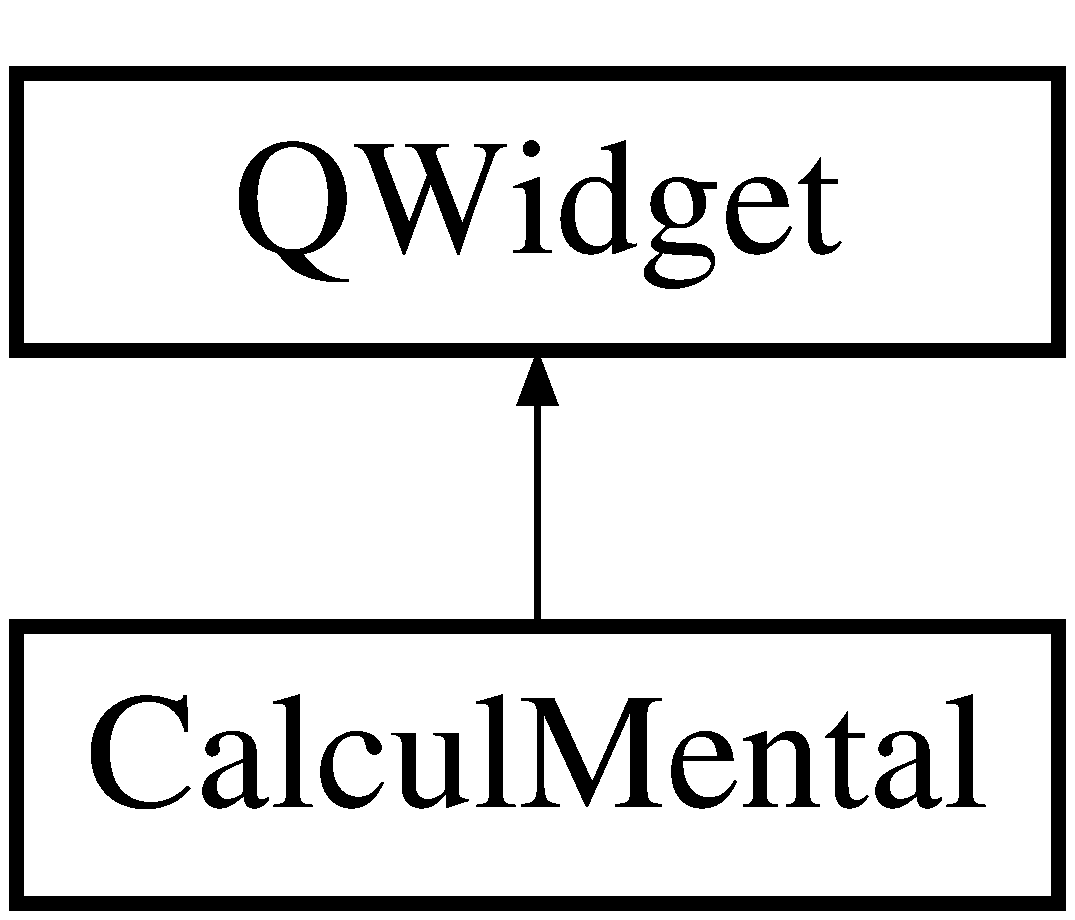
\includegraphics[height=2.000000cm]{class_calcul_mental}
\end{center}
\end{figure}
\subsection*{Public Slots}
\begin{DoxyCompactItemize}
\item 
\mbox{\Hypertarget{class_calcul_mental_a4f5f4f6818eaa9968900e94ea2ddbd87}\label{class_calcul_mental_a4f5f4f6818eaa9968900e94ea2ddbd87}} 
void \hyperlink{class_calcul_mental_a4f5f4f6818eaa9968900e94ea2ddbd87}{reset\+Score} ()
\begin{DoxyCompactList}\small\item\em Appui sur bouton reset score. \end{DoxyCompactList}\item 
\mbox{\Hypertarget{class_calcul_mental_aec1aa48cc17bdce965ea7d9aed0044ef}\label{class_calcul_mental_aec1aa48cc17bdce965ea7d9aed0044ef}} 
void \hyperlink{class_calcul_mental_aec1aa48cc17bdce965ea7d9aed0044ef}{disp\+New\+Calc} ()
\begin{DoxyCompactList}\small\item\em Appui sur bouton nouveau calcul. \end{DoxyCompactList}\item 
void \hyperlink{class_calcul_mental_ae74ebe9d8a7f8581ab2958a7987b7d5d}{submit\+Res} ()
\begin{DoxyCompactList}\small\item\em Appui sur bouton soumettre résultat. \end{DoxyCompactList}\end{DoxyCompactItemize}
\subsection*{Public Member Functions}
\begin{DoxyCompactItemize}
\item 
\mbox{\Hypertarget{class_calcul_mental_a1d00ff120d4375847d790991edd85059}\label{class_calcul_mental_a1d00ff120d4375847d790991edd85059}} 
\hyperlink{class_calcul_mental_a1d00ff120d4375847d790991edd85059}{Calcul\+Mental} (Q\+Widget $\ast$parent=nullptr)
\begin{DoxyCompactList}\small\item\em Constructeur et destructeur. \end{DoxyCompactList}\item 
\mbox{\Hypertarget{class_calcul_mental_a2c3a044640c58c0cc865e286334ce591}\label{class_calcul_mental_a2c3a044640c58c0cc865e286334ce591}} 
void \hyperlink{class_calcul_mental_a2c3a044640c58c0cc865e286334ce591}{set\+Score} (Q\+String p\+Score)
\begin{DoxyCompactList}\small\item\em S\+C\+O\+RE. \end{DoxyCompactList}\item 
\mbox{\Hypertarget{class_calcul_mental_abfcfd41b1b8b818352674c2565dc084f}\label{class_calcul_mental_abfcfd41b1b8b818352674c2565dc084f}} 
Q\+String {\bfseries get\+Score} (void)
\item 
\mbox{\Hypertarget{class_calcul_mental_a3d56b1b9c73714179370b3f0ca4420e9}\label{class_calcul_mental_a3d56b1b9c73714179370b3f0ca4420e9}} 
Q\+String \hyperlink{class_calcul_mental_a3d56b1b9c73714179370b3f0ca4420e9}{get\+Ope1} (void)
\begin{DoxyCompactList}\small\item\em Récupérer les opérandes en lettres \end{DoxyCompactList}\item 
\mbox{\Hypertarget{class_calcul_mental_afa5c299ddbe9c23c0c12deb7765c70f1}\label{class_calcul_mental_afa5c299ddbe9c23c0c12deb7765c70f1}} 
Q\+String {\bfseries get\+Ope2} (void)
\item 
\mbox{\Hypertarget{class_calcul_mental_ab838d242ea4101002bf72f26b18c261b}\label{class_calcul_mental_ab838d242ea4101002bf72f26b18c261b}} 
Q\+String \hyperlink{class_calcul_mental_ab838d242ea4101002bf72f26b18c261b}{get\+Operator} (void)
\begin{DoxyCompactList}\small\item\em Récupérer l\textquotesingle{}opérateur. \end{DoxyCompactList}\item 
\mbox{\Hypertarget{class_calcul_mental_a559ea88a8156df0f54761c4f0cc17144}\label{class_calcul_mental_a559ea88a8156df0f54761c4f0cc17144}} 
Q\+String \hyperlink{class_calcul_mental_a559ea88a8156df0f54761c4f0cc17144}{get\+Exp\+Res} (void)
\begin{DoxyCompactList}\small\item\em Récupérer le résultat de l\textquotesingle{}expression. \end{DoxyCompactList}\item 
\mbox{\Hypertarget{class_calcul_mental_a1078407e65b60debd469fbdd6b629366}\label{class_calcul_mental_a1078407e65b60debd469fbdd6b629366}} 
void \hyperlink{class_calcul_mental_a1078407e65b60debd469fbdd6b629366}{ask\+New\+Calc} (void)
\begin{DoxyCompactList}\small\item\em Demander un nouveau calcul au modèle. \end{DoxyCompactList}\item 
\mbox{\Hypertarget{class_calcul_mental_a85dd050ef2efa7c6440a1ba0595b6c2e}\label{class_calcul_mental_a85dd050ef2efa7c6440a1ba0595b6c2e}} 
bool \hyperlink{class_calcul_mental_a85dd050ef2efa7c6440a1ba0595b6c2e}{check\+Result} (Q\+String res\+Propose)
\begin{DoxyCompactList}\small\item\em Vérifier le resultat, et s\textquotesingle{}il est bon ajouter un point et demander un nouveau calcul. \end{DoxyCompactList}\item 
\mbox{\Hypertarget{class_calcul_mental_a24f15b92a313ab8ca872b0d495ce4852}\label{class_calcul_mental_a24f15b92a313ab8ca872b0d495ce4852}} 
void \hyperlink{class_calcul_mental_a24f15b92a313ab8ca872b0d495ce4852}{add\+Point} (void)
\begin{DoxyCompactList}\small\item\em Ajouter un point au score. \end{DoxyCompactList}\item 
\mbox{\Hypertarget{class_calcul_mental_ac56dfddc93f21f48beb2202940d7d005}\label{class_calcul_mental_ac56dfddc93f21f48beb2202940d7d005}} 
Q\+String \hyperlink{class_calcul_mental_ac56dfddc93f21f48beb2202940d7d005}{get\+Ope1\+Str} (void)
\begin{DoxyCompactList}\small\item\em Get les opérandes en lettres. \end{DoxyCompactList}\item 
\mbox{\Hypertarget{class_calcul_mental_afd4f24b373c7ba4fe2fa247819266096}\label{class_calcul_mental_afd4f24b373c7ba4fe2fa247819266096}} 
Q\+String {\bfseries get\+Ope2\+Str} (void)
\end{DoxyCompactItemize}


\subsection{Member Function Documentation}
\mbox{\Hypertarget{class_calcul_mental_ae74ebe9d8a7f8581ab2958a7987b7d5d}\label{class_calcul_mental_ae74ebe9d8a7f8581ab2958a7987b7d5d}} 
\index{Calcul\+Mental@{Calcul\+Mental}!submit\+Res@{submit\+Res}}
\index{submit\+Res@{submit\+Res}!Calcul\+Mental@{Calcul\+Mental}}
\subsubsection{\texorpdfstring{submit\+Res}{submitRes}}
{\footnotesize\ttfamily void Calcul\+Mental\+::submit\+Res (\begin{DoxyParamCaption}{ }\end{DoxyParamCaption})\hspace{0.3cm}{\ttfamily [slot]}}



Appui sur bouton soumettre résultat. 



 \subsubsection*{S\+L\+O\+TS }

The documentation for this class was generated from the following files\+:\begin{DoxyCompactItemize}
\item 
C\+:/\+Users/\+Jean-\/\+Loup/\+Documents/\+L3/\+Projet\+Malette\+Jeux/\+Q\+T/\+L\+W\+Robin/\+Learn\+With\+Robin\+Main/calculmental.\+h\item 
C\+:/\+Users/\+Jean-\/\+Loup/\+Documents/\+L3/\+Projet\+Malette\+Jeux/\+Q\+T/\+L\+W\+Robin/\+Learn\+With\+Robin\+Main/calculmental.\+cpp\end{DoxyCompactItemize}

\hypertarget{class_flags}{}\section{Flags Class Reference}
\label{class_flags}\index{Flags@{Flags}}
Inheritance diagram for Flags\+:\begin{figure}[H]
\begin{center}
\leavevmode
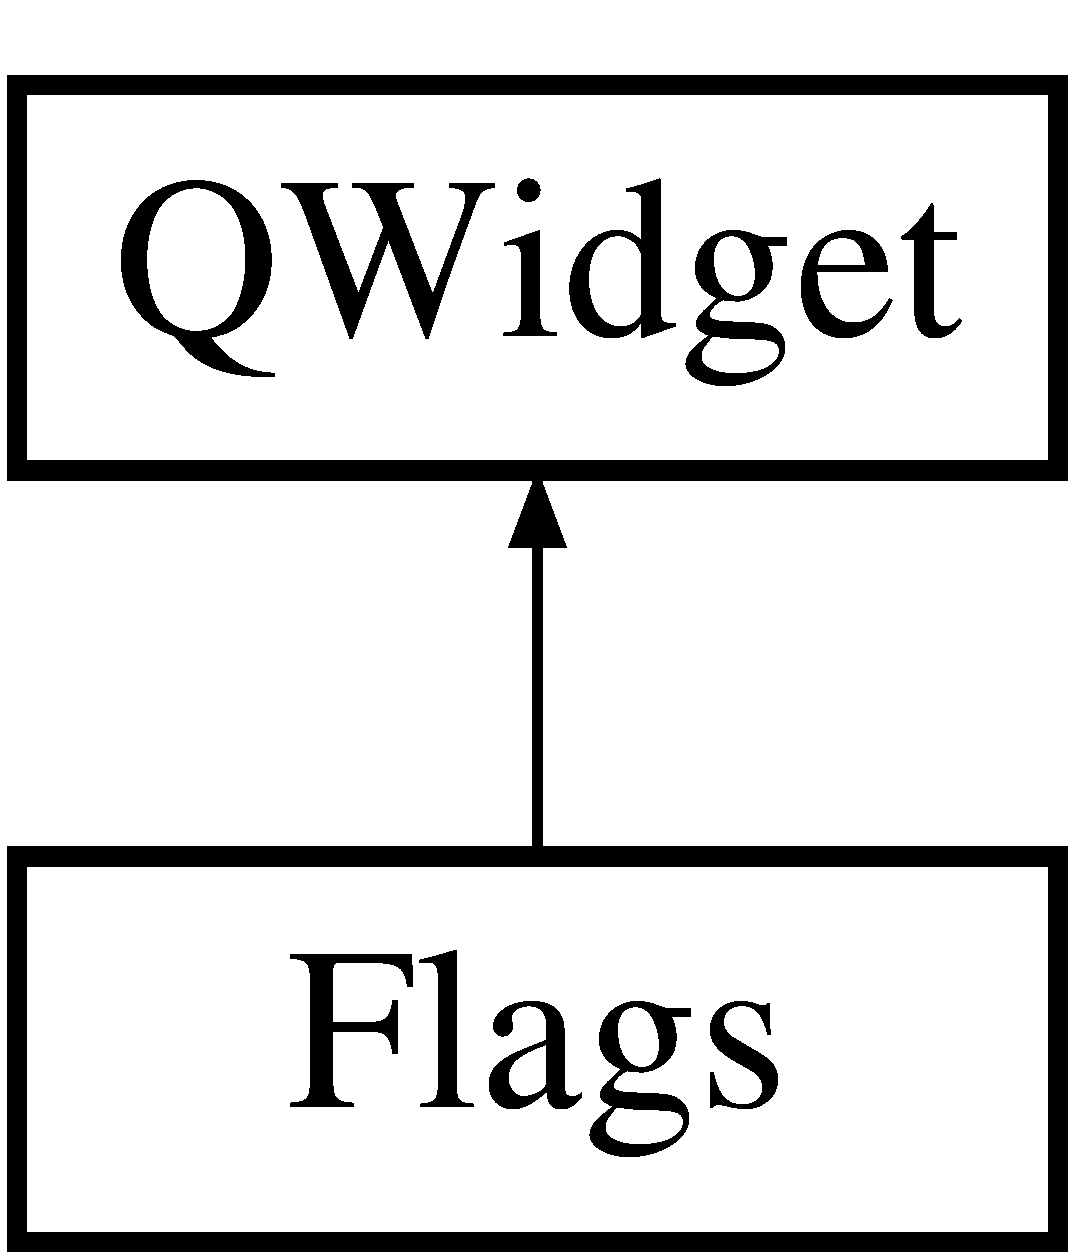
\includegraphics[height=2.000000cm]{class_flags}
\end{center}
\end{figure}
\subsection*{Public Member Functions}
\begin{DoxyCompactItemize}
\item 
\mbox{\Hypertarget{class_flags_a2efef25087c4092c8a79c64103a0093e}\label{class_flags_a2efef25087c4092c8a79c64103a0093e}} 
\hyperlink{class_flags_a2efef25087c4092c8a79c64103a0093e}{Flags} (Q\+Widget $\ast$parent=0)
\begin{DoxyCompactList}\small\item\em Constructeur et destructeur. \end{DoxyCompactList}\end{DoxyCompactItemize}


The documentation for this class was generated from the following files\+:\begin{DoxyCompactItemize}
\item 
C\+:/\+Users/\+Jean-\/\+Loup/\+Documents/\+L3/\+Projet\+Malette\+Jeux/\+Q\+T/\+L\+W\+Robin/\+Learn\+With\+Robin\+Main/flags.\+h\item 
C\+:/\+Users/\+Jean-\/\+Loup/\+Documents/\+L3/\+Projet\+Malette\+Jeux/\+Q\+T/\+L\+W\+Robin/\+Learn\+With\+Robin\+Main/flags.\+cpp\end{DoxyCompactItemize}

\hypertarget{class_main_menu}{}\section{Main\+Menu Class Reference}
\label{class_main_menu}\index{Main\+Menu@{Main\+Menu}}
Inheritance diagram for Main\+Menu\+:\begin{figure}[H]
\begin{center}
\leavevmode
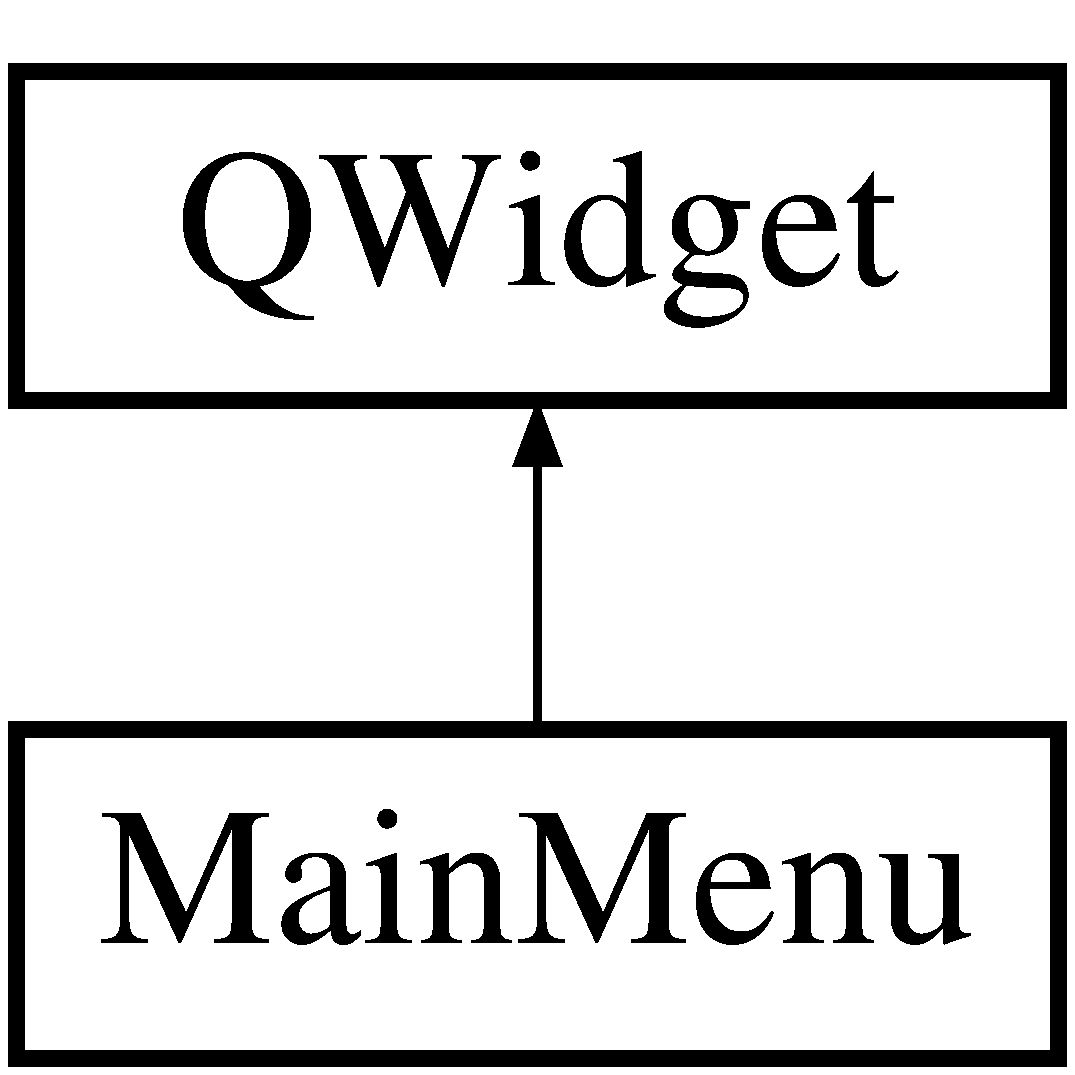
\includegraphics[height=2.000000cm]{class_main_menu}
\end{center}
\end{figure}
\subsection*{Public Slots}
\begin{DoxyCompactItemize}
\item 
void \hyperlink{class_main_menu_aecda91a1fbea29f928cf2334d5c5b1f3}{go\+For\+Calcul} (void)
\begin{DoxyCompactList}\small\item\em Appui sur le bouton calcul mental. \end{DoxyCompactList}\item 
\mbox{\Hypertarget{class_main_menu_a5f48134eefe4cc9e0a00922c4a09a647}\label{class_main_menu_a5f48134eefe4cc9e0a00922c4a09a647}} 
void \hyperlink{class_main_menu_a5f48134eefe4cc9e0a00922c4a09a647}{go\+For\+Simon} (void)
\begin{DoxyCompactList}\small\item\em Appui sur le bouton super simon. \end{DoxyCompactList}\item 
\mbox{\Hypertarget{class_main_menu_acc85e8df6cc1cf76fac3dfa998fbabc0}\label{class_main_menu_acc85e8df6cc1cf76fac3dfa998fbabc0}} 
void \hyperlink{class_main_menu_acc85e8df6cc1cf76fac3dfa998fbabc0}{go\+For\+Memory} (void)
\begin{DoxyCompactList}\small\item\em Appui sur le bouton memory. \end{DoxyCompactList}\end{DoxyCompactItemize}
\subsection*{Signals}
\begin{DoxyCompactItemize}
\item 
\mbox{\Hypertarget{class_main_menu_a598cb53314acb8fc35b5f2312db6e561}\label{class_main_menu_a598cb53314acb8fc35b5f2312db6e561}} 
void \hyperlink{class_main_menu_a598cb53314acb8fc35b5f2312db6e561}{clicked\+Calcul} (void)
\begin{DoxyCompactList}\small\item\em Signal pour lancer le jeu calcul mental. \end{DoxyCompactList}\item 
\mbox{\Hypertarget{class_main_menu_accfb16e9b9cbabbfd2460f8242648dd3}\label{class_main_menu_accfb16e9b9cbabbfd2460f8242648dd3}} 
void \hyperlink{class_main_menu_accfb16e9b9cbabbfd2460f8242648dd3}{clicked\+Simon} (void)
\begin{DoxyCompactList}\small\item\em Signal pour lancer le jeu super simon. \end{DoxyCompactList}\item 
\mbox{\Hypertarget{class_main_menu_a68da1f9eb32fa5536326328c0dead36f}\label{class_main_menu_a68da1f9eb32fa5536326328c0dead36f}} 
void \hyperlink{class_main_menu_a68da1f9eb32fa5536326328c0dead36f}{clicked\+Memory} (void)
\begin{DoxyCompactList}\small\item\em Signal pour lancer le jeu memory. \end{DoxyCompactList}\end{DoxyCompactItemize}
\subsection*{Public Member Functions}
\begin{DoxyCompactItemize}
\item 
\hyperlink{class_main_menu_a891bed1e0edb5492671c332cb89b7a9a}{Main\+Menu} (Q\+Widget $\ast$parent=nullptr)
\begin{DoxyCompactList}\small\item\em Constructeur et destructeur. \end{DoxyCompactList}\end{DoxyCompactItemize}


\subsection{Constructor \& Destructor Documentation}
\mbox{\Hypertarget{class_main_menu_a891bed1e0edb5492671c332cb89b7a9a}\label{class_main_menu_a891bed1e0edb5492671c332cb89b7a9a}} 
\index{Main\+Menu@{Main\+Menu}!Main\+Menu@{Main\+Menu}}
\index{Main\+Menu@{Main\+Menu}!Main\+Menu@{Main\+Menu}}
\subsubsection{\texorpdfstring{Main\+Menu()}{MainMenu()}}
{\footnotesize\ttfamily Main\+Menu\+::\+Main\+Menu (\begin{DoxyParamCaption}\item[{Q\+Widget $\ast$}]{parent = {\ttfamily nullptr} }\end{DoxyParamCaption})\hspace{0.3cm}{\ttfamily [explicit]}}



Constructeur et destructeur. 

\begin{DoxyRefDesc}{Test}
\item[\hyperlink{test__test000001}{Test}]nouvelle syntaxe connexion signal slot \end{DoxyRefDesc}


\subsection{Member Function Documentation}
\mbox{\Hypertarget{class_main_menu_aecda91a1fbea29f928cf2334d5c5b1f3}\label{class_main_menu_aecda91a1fbea29f928cf2334d5c5b1f3}} 
\index{Main\+Menu@{Main\+Menu}!go\+For\+Calcul@{go\+For\+Calcul}}
\index{go\+For\+Calcul@{go\+For\+Calcul}!Main\+Menu@{Main\+Menu}}
\subsubsection{\texorpdfstring{go\+For\+Calcul}{goForCalcul}}
{\footnotesize\ttfamily void Main\+Menu\+::go\+For\+Calcul (\begin{DoxyParamCaption}\item[{void}]{ }\end{DoxyParamCaption})\hspace{0.3cm}{\ttfamily [slot]}}



Appui sur le bouton calcul mental. 

\begin{DoxyNote}{Note}
on va garder la syntaxe go\+For, c\textquotesingle{}est bien \+:) 
\end{DoxyNote}


The documentation for this class was generated from the following files\+:\begin{DoxyCompactItemize}
\item 
C\+:/\+Users/\+Jean-\/\+Loup/\+Documents/\+L3/\+Projet\+Malette\+Jeux/\+Q\+T/\+L\+W\+Robin/\+Learn\+With\+Robin\+Main/mainmenu.\+h\item 
C\+:/\+Users/\+Jean-\/\+Loup/\+Documents/\+L3/\+Projet\+Malette\+Jeux/\+Q\+T/\+L\+W\+Robin/\+Learn\+With\+Robin\+Main/mainmenu.\+cpp\end{DoxyCompactItemize}

\hypertarget{class_memory}{}\section{Memory Class Reference}
\label{class_memory}\index{Memory@{Memory}}
Inheritance diagram for Memory\+:\begin{figure}[H]
\begin{center}
\leavevmode
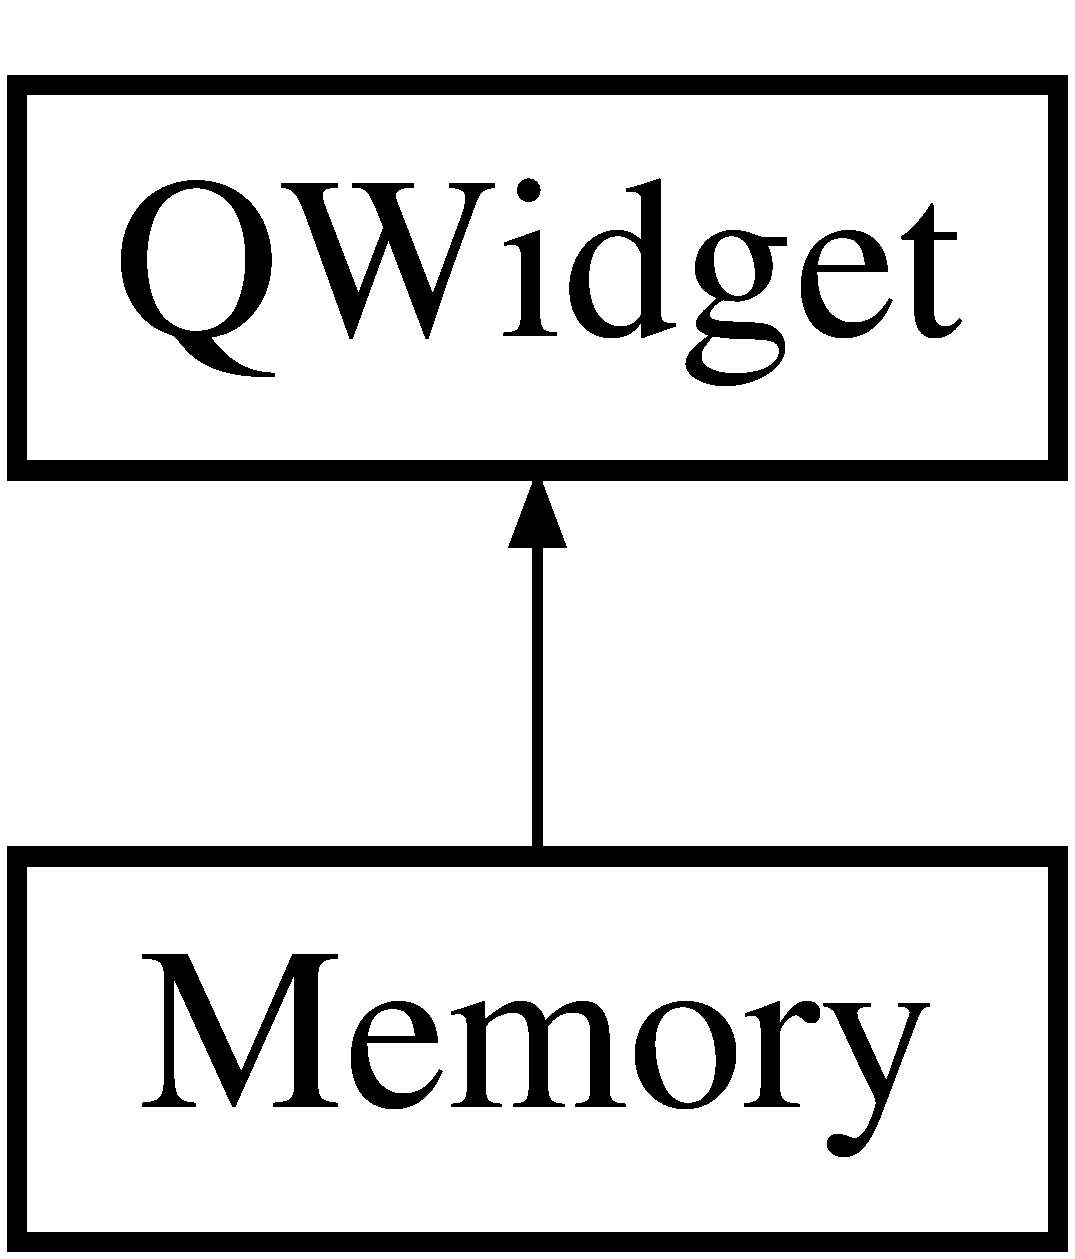
\includegraphics[height=2.000000cm]{class_memory}
\end{center}
\end{figure}
\subsection*{Public Slots}
\begin{DoxyCompactItemize}
\item 
\mbox{\Hypertarget{class_memory_af967fc9232b5f014ad2d5b020c463727}\label{class_memory_af967fc9232b5f014ad2d5b020c463727}} 
void \hyperlink{class_memory_af967fc9232b5f014ad2d5b020c463727}{carte\+Clic} (void)
\begin{DoxyCompactList}\small\item\em Clic sur une carte. \end{DoxyCompactList}\end{DoxyCompactItemize}
\subsection*{Signals}
\begin{DoxyCompactItemize}
\item 
\mbox{\Hypertarget{class_memory_a94744018f48144f6089011c74ee1a13b}\label{class_memory_a94744018f48144f6089011c74ee1a13b}} 
void \hyperlink{class_memory_a94744018f48144f6089011c74ee1a13b}{end\+Of\+Game} (std\+::pair$<$ std\+::string, int $>$ asso)
\begin{DoxyCompactList}\small\item\em fin du jeu \end{DoxyCompactList}\end{DoxyCompactItemize}
\subsection*{Public Member Functions}
\begin{DoxyCompactItemize}
\item 
\hyperlink{class_memory_a243eef3e0fd8d02131e3bcca0471c931}{Memory} (Q\+Widget $\ast$parent=0)
\begin{DoxyCompactList}\small\item\em Constructeur et destructeur. \end{DoxyCompactList}\item 
int \hyperlink{class_memory_a7c8b57775899a3782edcdf4da430ad61}{get\+Nb\+Cards} (void)
\begin{DoxyCompactList}\small\item\em Met à jour l\textquotesingle{}interface  void paint\+Event(\+Q\+Paint\+Event$\ast$);. \end{DoxyCompactList}\item 
void \hyperlink{class_memory_a296d041ffa5698d725cbf34257c8aeb3}{setup\+Card\+From\+Model} (int ind)
\begin{DoxyCompactList}\small\item\em Donner les informations. \end{DoxyCompactList}\item 
\mbox{\Hypertarget{class_memory_a21ee675074812b4fb7b56dd6795b229c}\label{class_memory_a21ee675074812b4fb7b56dd6795b229c}} 
std\+::string \hyperlink{class_memory_a21ee675074812b4fb7b56dd6795b229c}{get\+Card\+From\+Paire} (int paire)
\begin{DoxyCompactList}\small\item\em Retourne le nom de fichier attendu pour la paire. \end{DoxyCompactList}\item 
\mbox{\Hypertarget{class_memory_a162c70bd9a89e92e601c68ae51d78159}\label{class_memory_a162c70bd9a89e92e601c68ae51d78159}} 
int \hyperlink{class_memory_a162c70bd9a89e92e601c68ae51d78159}{get\+Indice\+From\+Name} (Q\+Push\+Button $\ast$but)
\begin{DoxyCompactList}\small\item\em Trouver l\textquotesingle{}indice de la carte depuis son nom. \end{DoxyCompactList}\item 
\mbox{\Hypertarget{class_memory_a8b2e64de3708d9ddf397517a668d813d}\label{class_memory_a8b2e64de3708d9ddf397517a668d813d}} 
void \hyperlink{class_memory_a8b2e64de3708d9ddf397517a668d813d}{close\+All\+Cards} (void)
\begin{DoxyCompactList}\small\item\em retourner toutes les cartes non appairées \end{DoxyCompactList}\item 
\mbox{\Hypertarget{class_memory_aee5f2b150b3b90ba1dd6ba7bf1b671a2}\label{class_memory_aee5f2b150b3b90ba1dd6ba7bf1b671a2}} 
void \hyperlink{class_memory_aee5f2b150b3b90ba1dd6ba7bf1b671a2}{send\+End\+Of\+Game} (void)
\begin{DoxyCompactList}\small\item\em Declencher fin du jeu. \end{DoxyCompactList}\item 
\mbox{\Hypertarget{class_memory_abfb41c91c7dd6166088a38b0689bc5e5}\label{class_memory_abfb41c91c7dd6166088a38b0689bc5e5}} 
bool \hyperlink{class_memory_abfb41c91c7dd6166088a38b0689bc5e5}{check\+End\+Of\+Game} (void)
\begin{DoxyCompactList}\small\item\em Verifier si fin du jeu. \end{DoxyCompactList}\end{DoxyCompactItemize}


\subsection{Constructor \& Destructor Documentation}
\mbox{\Hypertarget{class_memory_a243eef3e0fd8d02131e3bcca0471c931}\label{class_memory_a243eef3e0fd8d02131e3bcca0471c931}} 
\index{Memory@{Memory}!Memory@{Memory}}
\index{Memory@{Memory}!Memory@{Memory}}
\subsubsection{\texorpdfstring{Memory()}{Memory()}}
{\footnotesize\ttfamily Memory\+::\+Memory (\begin{DoxyParamCaption}\item[{Q\+Widget $\ast$}]{parent = {\ttfamily 0} }\end{DoxyParamCaption})\hspace{0.3cm}{\ttfamily [explicit]}}



Constructeur et destructeur. 

\begin{DoxyRefDesc}{Todo}
\item[\hyperlink{todo__todo000001}{Todo}]ordonner / ranger un peu cette fonction \end{DoxyRefDesc}


\begin{DoxyRefDesc}{Todo}
\item[\hyperlink{todo__todo000002}{Todo}]faire en sorte de régler le nombre de cartes selon la difficulté \end{DoxyRefDesc}


\begin{DoxyRefDesc}{Todo}
\item[\hyperlink{todo__todo000003}{Todo}]gérer le nombre de lignes et colonnes par rapport au nombre de cartes par exemple avec une approche de la racine carrée par la valeur inférieure pour les lignes, puis continuer à remplir dans les cases en revenant à la ligne à chaque fin de ligne, jusqu\textquotesingle{}à l\textquotesingle{}écoulement des cartes \end{DoxyRefDesc}


\subsection{Member Function Documentation}
\mbox{\Hypertarget{class_memory_a7c8b57775899a3782edcdf4da430ad61}\label{class_memory_a7c8b57775899a3782edcdf4da430ad61}} 
\index{Memory@{Memory}!get\+Nb\+Cards@{get\+Nb\+Cards}}
\index{get\+Nb\+Cards@{get\+Nb\+Cards}!Memory@{Memory}}
\subsubsection{\texorpdfstring{get\+Nb\+Cards()}{getNbCards()}}
{\footnotesize\ttfamily int Memory\+::get\+Nb\+Cards (\begin{DoxyParamCaption}\item[{void}]{ }\end{DoxyParamCaption})}



Met à jour l\textquotesingle{}interface  void paint\+Event(\+Q\+Paint\+Event$\ast$);. 

Récupère le nombre de cartes \begin{DoxyRefDesc}{Todo}
\item[\hyperlink{todo__todo000004}{Todo}]récupérer dans le modèle après \end{DoxyRefDesc}
\mbox{\Hypertarget{class_memory_a296d041ffa5698d725cbf34257c8aeb3}\label{class_memory_a296d041ffa5698d725cbf34257c8aeb3}} 
\index{Memory@{Memory}!setup\+Card\+From\+Model@{setup\+Card\+From\+Model}}
\index{setup\+Card\+From\+Model@{setup\+Card\+From\+Model}!Memory@{Memory}}
\subsubsection{\texorpdfstring{setup\+Card\+From\+Model()}{setupCardFromModel()}}
{\footnotesize\ttfamily void Memory\+::setup\+Card\+From\+Model (\begin{DoxyParamCaption}\item[{int}]{ind }\end{DoxyParamCaption})}



Donner les informations. 

Verifie si la carte est retournée ou non et lui attribue une stylesheet correspondant à cela en se basant pour son image si elle est retournée sur la paire du modele 

The documentation for this class was generated from the following files\+:\begin{DoxyCompactItemize}
\item 
C\+:/\+Users/\+Jean-\/\+Loup/\+Documents/\+L3/\+Projet\+Malette\+Jeux/\+Q\+T/\+L\+W\+Robin/\+Learn\+With\+Robin\+Main/memory.\+h\item 
C\+:/\+Users/\+Jean-\/\+Loup/\+Documents/\+L3/\+Projet\+Malette\+Jeux/\+Q\+T/\+L\+W\+Robin/\+Learn\+With\+Robin\+Main/memory.\+cpp\end{DoxyCompactItemize}

\hypertarget{class_memory_card}{}\section{Memory\+Card Class Reference}
\label{class_memory_card}\index{Memory\+Card@{Memory\+Card}}


Classe pour les cartes de memory.  




{\ttfamily \#include $<$modmemory.\+h$>$}

Inheritance diagram for Memory\+Card\+:\begin{figure}[H]
\begin{center}
\leavevmode
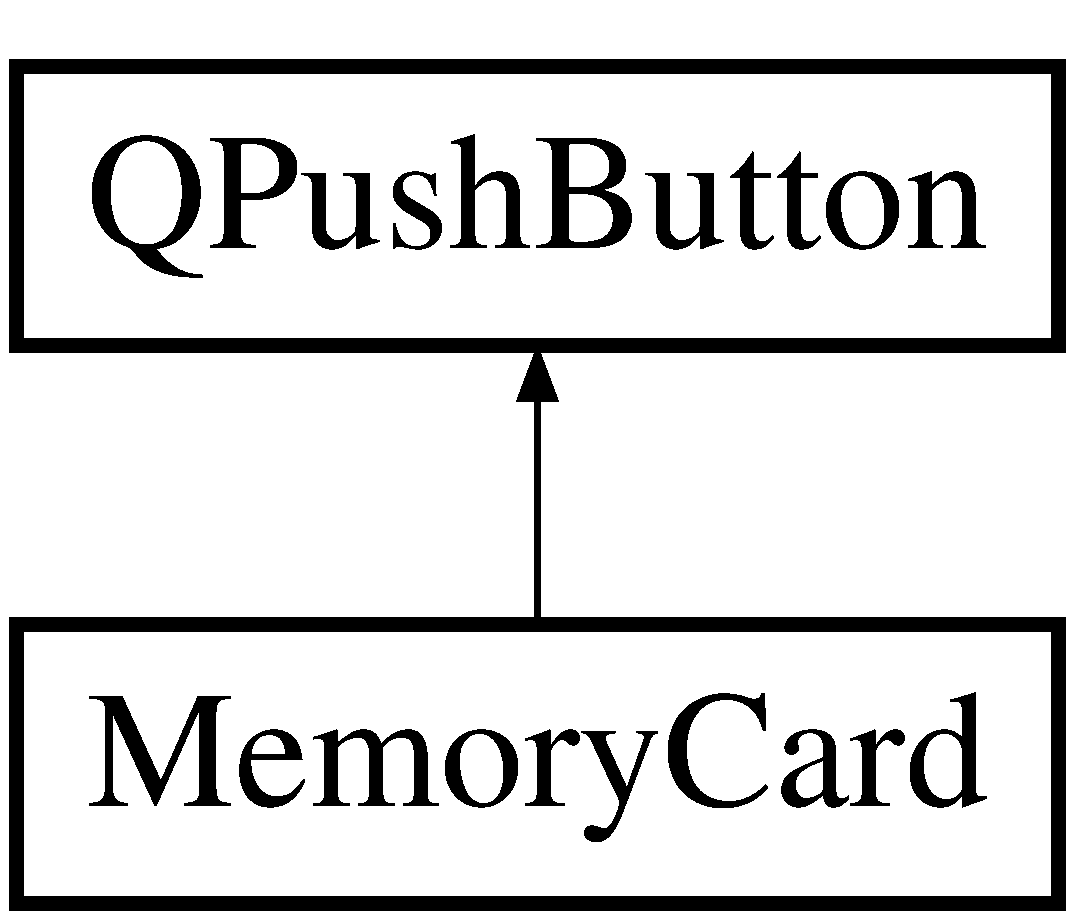
\includegraphics[height=2.000000cm]{class_memory_card}
\end{center}
\end{figure}
\subsection*{Public Member Functions}
\begin{DoxyCompactItemize}
\item 
\hyperlink{class_memory_card_a64380fa5fec0bcd01a1907804989ca9c}{Memory\+Card} (std\+::string \&path\+Back\+Card, std\+::string \&path\+Flip\+Card, int \&val\+\_\+pair)
\begin{DoxyCompactList}\small\item\em Constructeur. \end{DoxyCompactList}\item 
\mbox{\Hypertarget{class_memory_card_a3de3cef7b7af45dbf250435fb5004223}\label{class_memory_card_a3de3cef7b7af45dbf250435fb5004223}} 
\hyperlink{class_memory_card_a3de3cef7b7af45dbf250435fb5004223}{$\sim$\+Memory\+Card} (void)
\begin{DoxyCompactList}\small\item\em Destructeur. \end{DoxyCompactList}\item 
\mbox{\Hypertarget{class_memory_card_a1d6b3ba288249cbd619700cc4f4fddd3}\label{class_memory_card_a1d6b3ba288249cbd619700cc4f4fddd3}} 
int \hyperlink{class_memory_card_a1d6b3ba288249cbd619700cc4f4fddd3}{get\+Value\+Pair} (void)
\begin{DoxyCompactList}\small\item\em Donner l\textquotesingle{}index de la paire. \end{DoxyCompactList}\item 
\hyperlink{class_memory_card_a3d59bf204269e8b83a7eff862a838505}{Memory\+Card} (void)
\begin{DoxyCompactList}\small\item\em Constructeur par défaut. \end{DoxyCompactList}\item 
\hyperlink{class_memory_card_a682c2f65715e5e1bae9f0f04c361cddc}{Memory\+Card} (\hyperlink{class_memory_card}{Memory\+Card} \&)
\begin{DoxyCompactList}\small\item\em Constructeur par copie. \end{DoxyCompactList}\item 
\hyperlink{class_memory_card_ac34a1add168e88d58c5f864a35d4b136}{Memory\+Card} (int \&, int \&, bool, bool)
\begin{DoxyCompactList}\small\item\em Constructeur complet. \end{DoxyCompactList}\item 
\mbox{\Hypertarget{class_memory_card_a3de3cef7b7af45dbf250435fb5004223}\label{class_memory_card_a3de3cef7b7af45dbf250435fb5004223}} 
\hyperlink{class_memory_card_a3de3cef7b7af45dbf250435fb5004223}{$\sim$\+Memory\+Card} (void)
\begin{DoxyCompactList}\small\item\em Destructeur. \end{DoxyCompactList}\item 
\mbox{\Hypertarget{class_memory_card_ae46bae56b80b8a55957cf105240f8a50}\label{class_memory_card_ae46bae56b80b8a55957cf105240f8a50}} 
void \hyperlink{class_memory_card_ae46bae56b80b8a55957cf105240f8a50}{flip\+Card} (void)
\begin{DoxyCompactList}\small\item\em Inverse l\textquotesingle{}état retournee de la carte. \end{DoxyCompactList}\item 
\mbox{\Hypertarget{class_memory_card_ae704a33a0efe3fc47cff411154d0aa7f}\label{class_memory_card_ae704a33a0efe3fc47cff411154d0aa7f}} 
void \hyperlink{class_memory_card_ae704a33a0efe3fc47cff411154d0aa7f}{found\+Card} (void)
\begin{DoxyCompactList}\small\item\em Met associee à vrai. \end{DoxyCompactList}\item 
\mbox{\Hypertarget{class_memory_card_a17b81ae2bd924ae5430684ec02573aac}\label{class_memory_card_a17b81ae2bd924ae5430684ec02573aac}} 
void \hyperlink{class_memory_card_a17b81ae2bd924ae5430684ec02573aac}{set\+Indice} (int \&ind)
\begin{DoxyCompactList}\small\item\em Get-\/set l\textquotesingle{}indice d\textquotesingle{}une carte. \end{DoxyCompactList}\item 
\mbox{\Hypertarget{class_memory_card_a33e0dfc3a27e0342e21dd7aa0d01f3bc}\label{class_memory_card_a33e0dfc3a27e0342e21dd7aa0d01f3bc}} 
int {\bfseries get\+Indice} (void)
\item 
\mbox{\Hypertarget{class_memory_card_a0ceb17bd1ca14d7da5be66e7d5653d0b}\label{class_memory_card_a0ceb17bd1ca14d7da5be66e7d5653d0b}} 
void \hyperlink{class_memory_card_a0ceb17bd1ca14d7da5be66e7d5653d0b}{set\+Paire} (int \&pai)
\begin{DoxyCompactList}\small\item\em Get-\/set une paire. \end{DoxyCompactList}\item 
\mbox{\Hypertarget{class_memory_card_a61732d2d84d73b52d46506be8951d971}\label{class_memory_card_a61732d2d84d73b52d46506be8951d971}} 
int {\bfseries get\+Paire} (void)
\item 
\mbox{\Hypertarget{class_memory_card_a7ac054746ae11df4769bd97523e304fd}\label{class_memory_card_a7ac054746ae11df4769bd97523e304fd}} 
bool \hyperlink{class_memory_card_a7ac054746ae11df4769bd97523e304fd}{is\+Retournee} (void)
\begin{DoxyCompactList}\small\item\em Renvoie l\textquotesingle{}état de la carte (retournée ou non) \end{DoxyCompactList}\item 
\mbox{\Hypertarget{class_memory_card_aba6f7bf6100c8a0972732fd94f1523dd}\label{class_memory_card_aba6f7bf6100c8a0972732fd94f1523dd}} 
bool \hyperlink{class_memory_card_aba6f7bf6100c8a0972732fd94f1523dd}{is\+Associee} (void)
\begin{DoxyCompactList}\small\item\em Renvoie l\textquotesingle{}état de la paire (associée ou non) \end{DoxyCompactList}\end{DoxyCompactItemize}


\subsection{Detailed Description}
Classe pour les cartes de memory. 

\subsection{Constructor \& Destructor Documentation}
\mbox{\Hypertarget{class_memory_card_a64380fa5fec0bcd01a1907804989ca9c}\label{class_memory_card_a64380fa5fec0bcd01a1907804989ca9c}} 
\index{Memory\+Card@{Memory\+Card}!Memory\+Card@{Memory\+Card}}
\index{Memory\+Card@{Memory\+Card}!Memory\+Card@{Memory\+Card}}
\subsubsection{\texorpdfstring{Memory\+Card()}{MemoryCard()}\hspace{0.1cm}{\footnotesize\ttfamily [1/4]}}
{\footnotesize\ttfamily Memory\+Card\+::\+Memory\+Card (\begin{DoxyParamCaption}\item[{std\+::string \&}]{path\+Back\+Card,  }\item[{std\+::string \&}]{path\+Flip\+Card,  }\item[{int \&}]{val\+\_\+pair }\end{DoxyParamCaption})}



Constructeur. 


\begin{DoxyParams}{Parameters}
{\em path\+Back\+Card} & chemin vers l\textquotesingle{}image du dos de la carte \\
\hline
{\em path\+Flip\+Card} & chemin vers l\textquotesingle{}image de la face de la carte \\
\hline
{\em val\+\_\+pair} & index de la paire dans le tableau des paires \\
\hline
\end{DoxyParams}
\mbox{\Hypertarget{class_memory_card_a3d59bf204269e8b83a7eff862a838505}\label{class_memory_card_a3d59bf204269e8b83a7eff862a838505}} 
\index{Memory\+Card@{Memory\+Card}!Memory\+Card@{Memory\+Card}}
\index{Memory\+Card@{Memory\+Card}!Memory\+Card@{Memory\+Card}}
\subsubsection{\texorpdfstring{Memory\+Card()}{MemoryCard()}\hspace{0.1cm}{\footnotesize\ttfamily [2/4]}}
{\footnotesize\ttfamily Memory\+Card\+::\+Memory\+Card (\begin{DoxyParamCaption}\item[{void}]{ }\end{DoxyParamCaption})}



Constructeur par défaut. 

\hyperlink{class_memory_card}{Memory\+Card}. \mbox{\Hypertarget{class_memory_card_a682c2f65715e5e1bae9f0f04c361cddc}\label{class_memory_card_a682c2f65715e5e1bae9f0f04c361cddc}} 
\index{Memory\+Card@{Memory\+Card}!Memory\+Card@{Memory\+Card}}
\index{Memory\+Card@{Memory\+Card}!Memory\+Card@{Memory\+Card}}
\subsubsection{\texorpdfstring{Memory\+Card()}{MemoryCard()}\hspace{0.1cm}{\footnotesize\ttfamily [3/4]}}
{\footnotesize\ttfamily Memory\+Card\+::\+Memory\+Card (\begin{DoxyParamCaption}\item[{\hyperlink{class_memory_card}{Memory\+Card} \&}]{mem\+Cop }\end{DoxyParamCaption})}



Constructeur par copie. 

\hyperlink{class_memory_card}{Memory\+Card}. \mbox{\Hypertarget{class_memory_card_ac34a1add168e88d58c5f864a35d4b136}\label{class_memory_card_ac34a1add168e88d58c5f864a35d4b136}} 
\index{Memory\+Card@{Memory\+Card}!Memory\+Card@{Memory\+Card}}
\index{Memory\+Card@{Memory\+Card}!Memory\+Card@{Memory\+Card}}
\subsubsection{\texorpdfstring{Memory\+Card()}{MemoryCard()}\hspace{0.1cm}{\footnotesize\ttfamily [4/4]}}
{\footnotesize\ttfamily Memory\+Card\+::\+Memory\+Card (\begin{DoxyParamCaption}\item[{int \&}]{ind,  }\item[{int \&}]{pai,  }\item[{bool}]{ret,  }\item[{bool}]{asso }\end{DoxyParamCaption})}



Constructeur complet. 


\begin{DoxyParams}{Parameters}
{\em 1} & indice \\
\hline
{\em 2} & paire \\
\hline
{\em 3} & retournee \\
\hline
{\em 4} & associee \\
\hline
\end{DoxyParams}


The documentation for this class was generated from the following files\+:\begin{DoxyCompactItemize}
\item 
C\+:/\+Users/\+Jean-\/\+Loup/\+Documents/\+L3/\+Projet\+Malette\+Jeux/\+Q\+T/\+L\+W\+Robin/\+Learn\+With\+Robin\+Main/memoryaddons.\+h\item 
C\+:/\+Users/\+Jean-\/\+Loup/\+Documents/\+L3/\+Projet\+Malette\+Jeux/\+Q\+T/\+L\+W\+Robin/\+Learn\+With\+Robin\+Main/modmemory.\+h\item 
C\+:/\+Users/\+Jean-\/\+Loup/\+Documents/\+L3/\+Projet\+Malette\+Jeux/\+Q\+T/\+L\+W\+Robin/\+Learn\+With\+Robin\+Main/modmemory.\+cpp\end{DoxyCompactItemize}

\hypertarget{class_memory_index_cards}{}\section{Memory\+Index\+Cards Class Reference}
\label{class_memory_index_cards}\index{Memory\+Index\+Cards@{Memory\+Index\+Cards}}


{\ttfamily \#include $<$memoryaddons.\+h$>$}

\subsection*{Public Member Functions}
\begin{DoxyCompactItemize}
\item 
\hyperlink{class_memory_index_cards_a10ae71958cd423edde68dc41dd010a66}{Memory\+Index\+Cards} (std\+::string \&pathcsv)
\begin{DoxyCompactList}\small\item\em Constructeur à partir d\textquotesingle{}un fichier csv. \end{DoxyCompactList}\end{DoxyCompactItemize}


\subsection{Detailed Description}
\begin{DoxyRefDesc}{Todo}
\item[\hyperlink{todo__todo000005}{Todo}]il faudra un générateur de stylesheet efficace \end{DoxyRefDesc}


\subsection{Constructor \& Destructor Documentation}
\mbox{\Hypertarget{class_memory_index_cards_a10ae71958cd423edde68dc41dd010a66}\label{class_memory_index_cards_a10ae71958cd423edde68dc41dd010a66}} 
\index{Memory\+Index\+Cards@{Memory\+Index\+Cards}!Memory\+Index\+Cards@{Memory\+Index\+Cards}}
\index{Memory\+Index\+Cards@{Memory\+Index\+Cards}!Memory\+Index\+Cards@{Memory\+Index\+Cards}}
\subsubsection{\texorpdfstring{Memory\+Index\+Cards()}{MemoryIndexCards()}}
{\footnotesize\ttfamily Memory\+Index\+Cards\+::\+Memory\+Index\+Cards (\begin{DoxyParamCaption}\item[{std\+::string \&}]{pathcsv }\end{DoxyParamCaption})}



Constructeur à partir d\textquotesingle{}un fichier csv. 

\begin{DoxyRefDesc}{Todo}
\item[\hyperlink{todo__todo000006}{Todo}]implémenter \end{DoxyRefDesc}


The documentation for this class was generated from the following file\+:\begin{DoxyCompactItemize}
\item 
C\+:/\+Users/\+Jean-\/\+Loup/\+Documents/\+L3/\+Projet\+Malette\+Jeux/\+Q\+T/\+L\+W\+Robin/\+Learn\+With\+Robin\+Main/memoryaddons.\+h\end{DoxyCompactItemize}

\hypertarget{class_mod_calcul}{}\section{Mod\+Calcul Class Reference}
\label{class_mod_calcul}\index{Mod\+Calcul@{Mod\+Calcul}}
\subsection*{Public Types}
\begin{DoxyCompactItemize}
\item 
\mbox{\Hypertarget{class_mod_calcul_a6c7aa1fa9a9cf577567da286e26596ce}\label{class_mod_calcul_a6c7aa1fa9a9cf577567da286e26596ce}} 
enum \hyperlink{class_mod_calcul_a6c7aa1fa9a9cf577567da286e26596ce}{pos\+Set\+Op} \{ {\bfseries O\+P\+E\+\_\+\+A\+LL}, 
{\bfseries O\+P\+E\+\_\+\+E\+A\+SY}, 
{\bfseries O\+P\+E\+\_\+\+N\+O\+RM}
 \}\begin{DoxyCompactList}\small\item\em Possibilités set\+Operateurs. \end{DoxyCompactList}
\end{DoxyCompactItemize}
\subsection*{Public Member Functions}
\begin{DoxyCompactItemize}
\item 
\mbox{\Hypertarget{class_mod_calcul_ac5da8ccb4058c1c3aa3ee15a60572f23}\label{class_mod_calcul_ac5da8ccb4058c1c3aa3ee15a60572f23}} 
\hyperlink{class_mod_calcul_ac5da8ccb4058c1c3aa3ee15a60572f23}{Mod\+Calcul} (void)
\begin{DoxyCompactList}\small\item\em Constructeur et destructeur. \end{DoxyCompactList}\item 
\hyperlink{class_mod_calcul_a80ee3b9e056beb4942449219ac036e6e}{Mod\+Calcul} (const \hyperlink{class_mod_calcul}{Mod\+Calcul} \&mod\+To\+Copy)
\item 
\hyperlink{class_mod_calcul_ad10f52bb861bf4b76e12f5bba1d97b67}{Mod\+Calcul} (\hyperlink{class_mod_calcul}{Mod\+Calcul} $\ast$mod\+To\+Copy)
\item 
\mbox{\Hypertarget{class_mod_calcul_a28524d6936ea23d374b01d8b0f8feba2}\label{class_mod_calcul_a28524d6936ea23d374b01d8b0f8feba2}} 
\hyperlink{class_mod_calcul_a28524d6936ea23d374b01d8b0f8feba2}{Mod\+Calcul} (int bmin, int bmax, \hyperlink{class_mod_calcul_a6c7aa1fa9a9cf577567da286e26596ce}{pos\+Set\+Op} set\+Ope)
\begin{DoxyCompactList}\small\item\em Constructeur et initialisation du premier calcul. \end{DoxyCompactList}\item 
\mbox{\Hypertarget{class_mod_calcul_a3bc78a2a5165705dc3f15f516b6dc22c}\label{class_mod_calcul_a3bc78a2a5165705dc3f15f516b6dc22c}} 
void \hyperlink{class_mod_calcul_a3bc78a2a5165705dc3f15f516b6dc22c}{set\+Bornes} (int bmin, int bmax)
\begin{DoxyCompactList}\small\item\em Définir les bornes des chiffres proposés pour la somme. \end{DoxyCompactList}\item 
void \hyperlink{class_mod_calcul_ad6061decce032f0debf6fa79d153df5d}{ini\+Set\+Operateurs} (\hyperlink{class_mod_calcul_a6c7aa1fa9a9cf577567da286e26596ce}{pos\+Set\+Op} set\+Op)
\begin{DoxyCompactList}\small\item\em Définir quel set d\textquotesingle{}opérateurs employer. \end{DoxyCompactList}\item 
void \hyperlink{class_mod_calcul_ab725cb964df070cf7ccda5853ea918f2}{ini\+Calcul} (void)
\begin{DoxyCompactList}\small\item\em Créer un calcul. \end{DoxyCompactList}\item 
\mbox{\Hypertarget{class_mod_calcul_a0fbbf13959d04845c103e106e6c495dc}\label{class_mod_calcul_a0fbbf13959d04845c103e106e6c495dc}} 
int \hyperlink{class_mod_calcul_a0fbbf13959d04845c103e106e6c495dc}{get\+Operande1} (void)
\begin{DoxyCompactList}\small\item\em Donner les opérandes. \end{DoxyCompactList}\item 
\mbox{\Hypertarget{class_mod_calcul_ab48d9276a63761f6a034ed746d21df0b}\label{class_mod_calcul_ab48d9276a63761f6a034ed746d21df0b}} 
int {\bfseries get\+Operande2} (void)
\item 
\mbox{\Hypertarget{class_mod_calcul_a532a25b057812a683fccd87164818e58}\label{class_mod_calcul_a532a25b057812a683fccd87164818e58}} 
int \hyperlink{class_mod_calcul_a532a25b057812a683fccd87164818e58}{get\+Ope\+Min} (void)
\begin{DoxyCompactList}\small\item\em Donner les min et max. \end{DoxyCompactList}\item 
\mbox{\Hypertarget{class_mod_calcul_ad8e5ae82931e90554c3f253d7e013176}\label{class_mod_calcul_ad8e5ae82931e90554c3f253d7e013176}} 
int {\bfseries get\+Ope\+Max} (void)
\item 
\mbox{\Hypertarget{class_mod_calcul_abb295fd73af71d56b2ba3a7395336ec1}\label{class_mod_calcul_abb295fd73af71d56b2ba3a7395336ec1}} 
std\+::string \hyperlink{class_mod_calcul_abb295fd73af71d56b2ba3a7395336ec1}{get\+Operateur} (void)
\begin{DoxyCompactList}\small\item\em Donner l\textquotesingle{}opérateur. \end{DoxyCompactList}\item 
\mbox{\Hypertarget{class_mod_calcul_ab7ec5c33e373740b4096534b78198011}\label{class_mod_calcul_ab7ec5c33e373740b4096534b78198011}} 
int \hyperlink{class_mod_calcul_ab7ec5c33e373740b4096534b78198011}{get\+Result} (void)
\begin{DoxyCompactList}\small\item\em Donner le résultat. \end{DoxyCompactList}\item 
bool \hyperlink{class_mod_calcul_a66c4a1a155a2a74a53bba15967ef1bdb}{verif\+Res} (int prop)
\begin{DoxyCompactList}\small\item\em Verifier le résultat. \end{DoxyCompactList}\item 
void \hyperlink{class_mod_calcul_ab2fe81565c7084fa2c4344fce053eb14}{reset\+Score} (void)
\begin{DoxyCompactList}\small\item\em Gestion du score. \end{DoxyCompactList}\item 
\mbox{\Hypertarget{class_mod_calcul_a6d8cf463ce23eacb768e2ce8ef8e348a}\label{class_mod_calcul_a6d8cf463ce23eacb768e2ce8ef8e348a}} 
int {\bfseries get\+Score} (void)
\item 
\mbox{\Hypertarget{class_mod_calcul_ad10794443a0c0684912d1b22e3612bd3}\label{class_mod_calcul_ad10794443a0c0684912d1b22e3612bd3}} 
void {\bfseries set\+Score} (int nS)
\item 
\mbox{\Hypertarget{class_mod_calcul_a7e4594693f592c46b245f1aa1de31ce8}\label{class_mod_calcul_a7e4594693f592c46b245f1aa1de31ce8}} 
void {\bfseries one\+Point} (void)
\item 
std\+::string \hyperlink{class_mod_calcul_aa16185334bb48c8e312bd0b9148aa00d}{get\+Ope1\+Str} (void)
\begin{DoxyCompactList}\small\item\em Donner les nombres en toutes lettres. \end{DoxyCompactList}\item 
\mbox{\Hypertarget{class_mod_calcul_a77b55cb859fcae911e8d3d2521885ea5}\label{class_mod_calcul_a77b55cb859fcae911e8d3d2521885ea5}} 
std\+::string {\bfseries get\+Ope2\+Str} (void)
\end{DoxyCompactItemize}


\subsection{Constructor \& Destructor Documentation}
\mbox{\Hypertarget{class_mod_calcul_a80ee3b9e056beb4942449219ac036e6e}\label{class_mod_calcul_a80ee3b9e056beb4942449219ac036e6e}} 
\index{Mod\+Calcul@{Mod\+Calcul}!Mod\+Calcul@{Mod\+Calcul}}
\index{Mod\+Calcul@{Mod\+Calcul}!Mod\+Calcul@{Mod\+Calcul}}
\subsubsection{\texorpdfstring{Mod\+Calcul()}{ModCalcul()}\hspace{0.1cm}{\footnotesize\ttfamily [1/2]}}
{\footnotesize\ttfamily Mod\+Calcul\+::\+Mod\+Calcul (\begin{DoxyParamCaption}\item[{const \hyperlink{class_mod_calcul}{Mod\+Calcul} \&}]{mod\+To\+Copy }\end{DoxyParamCaption})}

\begin{DoxyNote}{Note}
ne va probablement pas être vraiment utilisé 
\end{DoxyNote}
\mbox{\Hypertarget{class_mod_calcul_ad10f52bb861bf4b76e12f5bba1d97b67}\label{class_mod_calcul_ad10f52bb861bf4b76e12f5bba1d97b67}} 
\index{Mod\+Calcul@{Mod\+Calcul}!Mod\+Calcul@{Mod\+Calcul}}
\index{Mod\+Calcul@{Mod\+Calcul}!Mod\+Calcul@{Mod\+Calcul}}
\subsubsection{\texorpdfstring{Mod\+Calcul()}{ModCalcul()}\hspace{0.1cm}{\footnotesize\ttfamily [2/2]}}
{\footnotesize\ttfamily Mod\+Calcul\+::\+Mod\+Calcul (\begin{DoxyParamCaption}\item[{\hyperlink{class_mod_calcul}{Mod\+Calcul} $\ast$}]{ptr\+Mod }\end{DoxyParamCaption})}

\begin{DoxyNote}{Note}
probablement pas non plus 
\end{DoxyNote}


\subsection{Member Function Documentation}
\mbox{\Hypertarget{class_mod_calcul_aa16185334bb48c8e312bd0b9148aa00d}\label{class_mod_calcul_aa16185334bb48c8e312bd0b9148aa00d}} 
\index{Mod\+Calcul@{Mod\+Calcul}!get\+Ope1\+Str@{get\+Ope1\+Str}}
\index{get\+Ope1\+Str@{get\+Ope1\+Str}!Mod\+Calcul@{Mod\+Calcul}}
\subsubsection{\texorpdfstring{get\+Ope1\+Str()}{getOpe1Str()}}
{\footnotesize\ttfamily std\+::string Mod\+Calcul\+::get\+Ope1\+Str (\begin{DoxyParamCaption}\item[{void}]{ }\end{DoxyParamCaption})}



Donner les nombres en toutes lettres. 

\begin{DoxyRefDesc}{Todo}
\item[\hyperlink{todo__todo000009}{Todo}]implémenter \end{DoxyRefDesc}
\mbox{\Hypertarget{class_mod_calcul_ab725cb964df070cf7ccda5853ea918f2}\label{class_mod_calcul_ab725cb964df070cf7ccda5853ea918f2}} 
\index{Mod\+Calcul@{Mod\+Calcul}!ini\+Calcul@{ini\+Calcul}}
\index{ini\+Calcul@{ini\+Calcul}!Mod\+Calcul@{Mod\+Calcul}}
\subsubsection{\texorpdfstring{ini\+Calcul()}{iniCalcul()}}
{\footnotesize\ttfamily void Mod\+Calcul\+::ini\+Calcul (\begin{DoxyParamCaption}\item[{void}]{ }\end{DoxyParamCaption})}



Créer un calcul. 

Creer un calcul. \mbox{\Hypertarget{class_mod_calcul_ad6061decce032f0debf6fa79d153df5d}\label{class_mod_calcul_ad6061decce032f0debf6fa79d153df5d}} 
\index{Mod\+Calcul@{Mod\+Calcul}!ini\+Set\+Operateurs@{ini\+Set\+Operateurs}}
\index{ini\+Set\+Operateurs@{ini\+Set\+Operateurs}!Mod\+Calcul@{Mod\+Calcul}}
\subsubsection{\texorpdfstring{ini\+Set\+Operateurs()}{iniSetOperateurs()}}
{\footnotesize\ttfamily void Mod\+Calcul\+::ini\+Set\+Operateurs (\begin{DoxyParamCaption}\item[{\hyperlink{class_mod_calcul_a6c7aa1fa9a9cf577567da286e26596ce}{pos\+Set\+Op}}]{set\+Op }\end{DoxyParamCaption})}



Définir quel set d\textquotesingle{}opérateurs employer. 

\begin{DoxyRefDesc}{Todo}
\item[\hyperlink{todo__todo000008}{Todo}]gérer ça \end{DoxyRefDesc}

\begin{DoxyParams}{Parameters}
{\em set\+Op} & parmi O\+P\+E\+\_\+\+A\+LL, O\+P\+E\+\_\+\+E\+A\+SY, O\+P\+E\+\_\+\+N\+O\+RM\\
\hline
\end{DoxyParams}
Définir quel set d\textquotesingle{}opérateurs employer \begin{DoxyRefDesc}{Todo}
\item[\hyperlink{todo__todo000007}{Todo}]gérer ça \end{DoxyRefDesc}

\begin{DoxyParams}{Parameters}
{\em set\+Op} & parmi O\+P\+E\+\_\+\+A\+LL, O\+P\+E\+\_\+\+E\+A\+SY, O\+P\+E\+\_\+\+N\+O\+RM \\
\hline
\end{DoxyParams}
\mbox{\Hypertarget{class_mod_calcul_ab2fe81565c7084fa2c4344fce053eb14}\label{class_mod_calcul_ab2fe81565c7084fa2c4344fce053eb14}} 
\index{Mod\+Calcul@{Mod\+Calcul}!reset\+Score@{reset\+Score}}
\index{reset\+Score@{reset\+Score}!Mod\+Calcul@{Mod\+Calcul}}
\subsubsection{\texorpdfstring{reset\+Score()}{resetScore()}}
{\footnotesize\ttfamily void Mod\+Calcul\+::reset\+Score (\begin{DoxyParamCaption}\item[{void}]{ }\end{DoxyParamCaption})}



Gestion du score. 

Gestion du score (test) \mbox{\Hypertarget{class_mod_calcul_a66c4a1a155a2a74a53bba15967ef1bdb}\label{class_mod_calcul_a66c4a1a155a2a74a53bba15967ef1bdb}} 
\index{Mod\+Calcul@{Mod\+Calcul}!verif\+Res@{verif\+Res}}
\index{verif\+Res@{verif\+Res}!Mod\+Calcul@{Mod\+Calcul}}
\subsubsection{\texorpdfstring{verif\+Res()}{verifRes()}}
{\footnotesize\ttfamily bool Mod\+Calcul\+::verif\+Res (\begin{DoxyParamCaption}\item[{int}]{prop }\end{DoxyParamCaption})}



Verifier le résultat. 

Verification du résultat. 

The documentation for this class was generated from the following files\+:\begin{DoxyCompactItemize}
\item 
C\+:/\+Users/\+Jean-\/\+Loup/\+Documents/\+L3/\+Projet\+Malette\+Jeux/\+Q\+T/\+L\+W\+Robin/\+Learn\+With\+Robin\+Main/modcalcul.\+h\item 
C\+:/\+Users/\+Jean-\/\+Loup/\+Documents/\+L3/\+Projet\+Malette\+Jeux/\+Q\+T/\+L\+W\+Robin/\+Learn\+With\+Robin\+Main/modcalcul.\+cpp\end{DoxyCompactItemize}

\hypertarget{class_mod_flags}{}\section{Mod\+Flags Class Reference}
\label{class_mod_flags}\index{Mod\+Flags@{Mod\+Flags}}
\subsection*{Public Member Functions}
\begin{DoxyCompactItemize}
\item 
\mbox{\Hypertarget{class_mod_flags_a5d6e32a267ab2ef7bc4b63522b0db027}\label{class_mod_flags_a5d6e32a267ab2ef7bc4b63522b0db027}} 
\hyperlink{class_mod_flags_a5d6e32a267ab2ef7bc4b63522b0db027}{Mod\+Flags} ()
\begin{DoxyCompactList}\small\item\em Constructeur. \end{DoxyCompactList}\end{DoxyCompactItemize}


The documentation for this class was generated from the following files\+:\begin{DoxyCompactItemize}
\item 
C\+:/\+Users/\+Jean-\/\+Loup/\+Documents/\+L3/\+Projet\+Malette\+Jeux/\+Q\+T/\+L\+W\+Robin/\+Learn\+With\+Robin\+Main/modflags.\+h\item 
C\+:/\+Users/\+Jean-\/\+Loup/\+Documents/\+L3/\+Projet\+Malette\+Jeux/\+Q\+T/\+L\+W\+Robin/\+Learn\+With\+Robin\+Main/modflags.\+cpp\end{DoxyCompactItemize}

\hypertarget{class_mod_memory}{}\section{Mod\+Memory Class Reference}
\label{class_mod_memory}\index{Mod\+Memory@{Mod\+Memory}}


{\ttfamily \#include $<$modmemory.\+h$>$}

\subsection*{Public Member Functions}
\begin{DoxyCompactItemize}
\item 
\hyperlink{class_mod_memory_a8604678a120d5f8e430d5d2248a44e36}{Mod\+Memory} ()
\begin{DoxyCompactList}\small\item\em Constructeur. \end{DoxyCompactList}\item 
\hyperlink{class_mod_memory_a77d39288e861c84edcfa760170fbc44d}{$\sim$\+Mod\+Memory} ()
\begin{DoxyCompactList}\small\item\em Destructeur. \end{DoxyCompactList}\item 
void \hyperlink{class_mod_memory_ad85f5a28220e641195215e705a928fb1}{shuffle\+Cards} (void)
\begin{DoxyCompactList}\small\item\em Mélanger les cartes dans le vecteur. \end{DoxyCompactList}\item 
bool \hyperlink{class_mod_memory_a67247c021d8bf91192c2c32c1eb560ad}{card\+Is\+Open} (int \&)
\begin{DoxyCompactList}\small\item\em Vérifie si la carte est retournée. \end{DoxyCompactList}\item 
void \hyperlink{class_mod_memory_a5886105416521e463eeaf732e8a0f6fe}{open\+Card} (int \&)
\begin{DoxyCompactList}\small\item\em Retourner une carte face visible. \end{DoxyCompactList}\item 
void \hyperlink{class_mod_memory_a4e6581fef7b3adbad429bf4c39d38e88}{close\+Cards} (void)
\begin{DoxyCompactList}\small\item\em Retourne les cartes de flippedcards face cachée. \end{DoxyCompactList}\item 
\mbox{\Hypertarget{class_mod_memory_ab037bba20af618761450a5bf4e221d4b}\label{class_mod_memory_ab037bba20af618761450a5bf4e221d4b}} 
bool \hyperlink{class_mod_memory_ab037bba20af618761450a5bf4e221d4b}{check\+Cards} (int \&, int \&)
\begin{DoxyCompactList}\small\item\em Vérifier si les cartes appartiennent à la même paire. \end{DoxyCompactList}\item 
int \hyperlink{class_mod_memory_a2ea383b6a13143c4f1f5fa9534e6faa6}{get\+Indice\+Carte} (int \&)
\begin{DoxyCompactList}\small\item\em Indice de la carte. \end{DoxyCompactList}\item 
\mbox{\Hypertarget{class_mod_memory_a0f00b2aabc36bccd1eae114917b0bdc3}\label{class_mod_memory_a0f00b2aabc36bccd1eae114917b0bdc3}} 
int \hyperlink{class_mod_memory_a0f00b2aabc36bccd1eae114917b0bdc3}{get\+Paire\+Carte} (int \&)
\begin{DoxyCompactList}\small\item\em Paire de la carte. \end{DoxyCompactList}\item 
\mbox{\Hypertarget{class_mod_memory_a01b946e68364a820b65e4681b4b87ed8}\label{class_mod_memory_a01b946e68364a820b65e4681b4b87ed8}} 
bool \hyperlink{class_mod_memory_a01b946e68364a820b65e4681b4b87ed8}{card\+Is\+Paired} (int \&)
\begin{DoxyCompactList}\small\item\em Vérifie si la carte est associée. \end{DoxyCompactList}\item 
\mbox{\Hypertarget{class_mod_memory_a42de695b99429f9a9461db78b2375e3a}\label{class_mod_memory_a42de695b99429f9a9461db78b2375e3a}} 
int \hyperlink{class_mod_memory_a42de695b99429f9a9461db78b2375e3a}{get\+Nb\+Cartes\+Retournees} (void)
\begin{DoxyCompactList}\small\item\em Getter. \end{DoxyCompactList}\item 
\mbox{\Hypertarget{class_mod_memory_a00449888edb65708081e0e074391a28c}\label{class_mod_memory_a00449888edb65708081e0e074391a28c}} 
std\+::pair$<$ int, int $>$ \hyperlink{class_mod_memory_a00449888edb65708081e0e074391a28c}{get\+Flipped\+Cards} (void)
\begin{DoxyCompactList}\small\item\em Getter de la paire de cartes retournées. \end{DoxyCompactList}\item 
\mbox{\Hypertarget{class_mod_memory_ada71dd41fee113c35c644f4c2e335096}\label{class_mod_memory_ada71dd41fee113c35c644f4c2e335096}} 
int \hyperlink{class_mod_memory_ada71dd41fee113c35c644f4c2e335096}{get\+Nb\+Cartes\+Restantes} (void)
\begin{DoxyCompactList}\small\item\em Getter. \end{DoxyCompactList}\end{DoxyCompactItemize}


\subsection{Detailed Description}
Classe du modèle 

\subsection{Constructor \& Destructor Documentation}
\mbox{\Hypertarget{class_mod_memory_a8604678a120d5f8e430d5d2248a44e36}\label{class_mod_memory_a8604678a120d5f8e430d5d2248a44e36}} 
\index{Mod\+Memory@{Mod\+Memory}!Mod\+Memory@{Mod\+Memory}}
\index{Mod\+Memory@{Mod\+Memory}!Mod\+Memory@{Mod\+Memory}}
\subsubsection{\texorpdfstring{Mod\+Memory()}{ModMemory()}}
{\footnotesize\ttfamily Mod\+Memory\+::\+Mod\+Memory (\begin{DoxyParamCaption}{ }\end{DoxyParamCaption})}



Constructeur. 

\hyperlink{class_mod_memory}{Mod\+Memory}. \mbox{\Hypertarget{class_mod_memory_a77d39288e861c84edcfa760170fbc44d}\label{class_mod_memory_a77d39288e861c84edcfa760170fbc44d}} 
\index{Mod\+Memory@{Mod\+Memory}!````~Mod\+Memory@{$\sim$\+Mod\+Memory}}
\index{````~Mod\+Memory@{$\sim$\+Mod\+Memory}!Mod\+Memory@{Mod\+Memory}}
\subsubsection{\texorpdfstring{$\sim$\+Mod\+Memory()}{~ModMemory()}}
{\footnotesize\ttfamily Mod\+Memory\+::$\sim$\+Mod\+Memory (\begin{DoxyParamCaption}{ }\end{DoxyParamCaption})}



Destructeur. 

\begin{DoxyRefDesc}{Todo}
\item[\hyperlink{todo__todo000013}{Todo}]supprimer contenu des vecteurs et les vider \end{DoxyRefDesc}


\subsection{Member Function Documentation}
\mbox{\Hypertarget{class_mod_memory_a67247c021d8bf91192c2c32c1eb560ad}\label{class_mod_memory_a67247c021d8bf91192c2c32c1eb560ad}} 
\index{Mod\+Memory@{Mod\+Memory}!card\+Is\+Open@{card\+Is\+Open}}
\index{card\+Is\+Open@{card\+Is\+Open}!Mod\+Memory@{Mod\+Memory}}
\subsubsection{\texorpdfstring{card\+Is\+Open()}{cardIsOpen()}}
{\footnotesize\ttfamily bool Mod\+Memory\+::card\+Is\+Open (\begin{DoxyParamCaption}\item[{int \&}]{ind }\end{DoxyParamCaption})}



Vérifie si la carte est retournée. 

\begin{DoxyWarning}{Warning}
Tous les indices demandés sour forme d\textquotesingle{}int sont les indice du vecteur, pas les attributs indices des Memory\+Cards elles-\/mêmes 
\end{DoxyWarning}
\mbox{\Hypertarget{class_mod_memory_a4e6581fef7b3adbad429bf4c39d38e88}\label{class_mod_memory_a4e6581fef7b3adbad429bf4c39d38e88}} 
\index{Mod\+Memory@{Mod\+Memory}!close\+Cards@{close\+Cards}}
\index{close\+Cards@{close\+Cards}!Mod\+Memory@{Mod\+Memory}}
\subsubsection{\texorpdfstring{close\+Cards()}{closeCards()}}
{\footnotesize\ttfamily void Mod\+Memory\+::close\+Cards (\begin{DoxyParamCaption}\item[{void}]{ }\end{DoxyParamCaption})}



Retourne les cartes de flippedcards face cachée. 

\begin{DoxyRefDesc}{Todo}
\item[\hyperlink{todo__todo000014}{Todo}]C\+O\+M\+P\+L\+E\+T\+ER en retournant les trucs de flipped card et verifier qu\textquotesingle{}on ne manipule pas flippedcard dans les methodes ou l\textquotesingle{}on devrait manipuler cards\end{DoxyRefDesc}


\begin{DoxyRefDesc}{Todo}
\item[\hyperlink{todo__todo000015}{Todo}]arreter d\textquotesingle{}etre malade \end{DoxyRefDesc}
\mbox{\Hypertarget{class_mod_memory_a2ea383b6a13143c4f1f5fa9534e6faa6}\label{class_mod_memory_a2ea383b6a13143c4f1f5fa9534e6faa6}} 
\index{Mod\+Memory@{Mod\+Memory}!get\+Indice\+Carte@{get\+Indice\+Carte}}
\index{get\+Indice\+Carte@{get\+Indice\+Carte}!Mod\+Memory@{Mod\+Memory}}
\subsubsection{\texorpdfstring{get\+Indice\+Carte()}{getIndiceCarte()}}
{\footnotesize\ttfamily int Mod\+Memory\+::get\+Indice\+Carte (\begin{DoxyParamCaption}\item[{int \&}]{ind }\end{DoxyParamCaption})}



Indice de la carte. 

Utile seulement pour le shuffle \mbox{\Hypertarget{class_mod_memory_a5886105416521e463eeaf732e8a0f6fe}\label{class_mod_memory_a5886105416521e463eeaf732e8a0f6fe}} 
\index{Mod\+Memory@{Mod\+Memory}!open\+Card@{open\+Card}}
\index{open\+Card@{open\+Card}!Mod\+Memory@{Mod\+Memory}}
\subsubsection{\texorpdfstring{open\+Card()}{openCard()}}
{\footnotesize\ttfamily void Mod\+Memory\+::open\+Card (\begin{DoxyParamCaption}\item[{int \&}]{ind }\end{DoxyParamCaption})}



Retourner une carte face visible. 

L\textquotesingle{}ajoute a la paire flipped\+Cards \mbox{\Hypertarget{class_mod_memory_ad85f5a28220e641195215e705a928fb1}\label{class_mod_memory_ad85f5a28220e641195215e705a928fb1}} 
\index{Mod\+Memory@{Mod\+Memory}!shuffle\+Cards@{shuffle\+Cards}}
\index{shuffle\+Cards@{shuffle\+Cards}!Mod\+Memory@{Mod\+Memory}}
\subsubsection{\texorpdfstring{shuffle\+Cards()}{shuffleCards()}}
{\footnotesize\ttfamily void Mod\+Memory\+::shuffle\+Cards (\begin{DoxyParamCaption}\item[{void}]{ }\end{DoxyParamCaption})}



Mélanger les cartes dans le vecteur. 

Principe \+: la vue va associer les cartes de son vecteur avec celles du modèle en prenant leurs indices dans leurs vecteurs respectifs, et le modèle va communiquer les informations des Memory\+Cards, mélangées donc. Tout ça pour dire que pas besoin de mélanger ou synchroniser la vue et le modèle entre eux.

En somme, le shuffle attribue les paires 

The documentation for this class was generated from the following files\+:\begin{DoxyCompactItemize}
\item 
C\+:/\+Users/\+Jean-\/\+Loup/\+Documents/\+L3/\+Projet\+Malette\+Jeux/\+Q\+T/\+L\+W\+Robin/\+Learn\+With\+Robin\+Main/modmemory.\+h\item 
C\+:/\+Users/\+Jean-\/\+Loup/\+Documents/\+L3/\+Projet\+Malette\+Jeux/\+Q\+T/\+L\+W\+Robin/\+Learn\+With\+Robin\+Main/modmemory.\+cpp\end{DoxyCompactItemize}

\hypertarget{class_mod_point_and_click}{}\section{Mod\+Point\+And\+Click Class Reference}
\label{class_mod_point_and_click}\index{Mod\+Point\+And\+Click@{Mod\+Point\+And\+Click}}
\subsection*{Public Member Functions}
\begin{DoxyCompactItemize}
\item 
\mbox{\Hypertarget{class_mod_point_and_click_a4867dd40a30d08034b7df13d67076e10}\label{class_mod_point_and_click_a4867dd40a30d08034b7df13d67076e10}} 
\hyperlink{class_mod_point_and_click_a4867dd40a30d08034b7df13d67076e10}{Mod\+Point\+And\+Click} ()
\begin{DoxyCompactList}\small\item\em Constructeur. \end{DoxyCompactList}\end{DoxyCompactItemize}


The documentation for this class was generated from the following files\+:\begin{DoxyCompactItemize}
\item 
C\+:/\+Users/\+Jean-\/\+Loup/\+Documents/\+L3/\+Projet\+Malette\+Jeux/\+Q\+T/\+L\+W\+Robin/\+Learn\+With\+Robin\+Main/modpointandclick.\+h\item 
C\+:/\+Users/\+Jean-\/\+Loup/\+Documents/\+L3/\+Projet\+Malette\+Jeux/\+Q\+T/\+L\+W\+Robin/\+Learn\+With\+Robin\+Main/modpointandclick.\+cpp\end{DoxyCompactItemize}

\hypertarget{class_mod_puzzle}{}\section{Mod\+Puzzle Class Reference}
\label{class_mod_puzzle}\index{Mod\+Puzzle@{Mod\+Puzzle}}
\subsection*{Public Member Functions}
\begin{DoxyCompactItemize}
\item 
\mbox{\Hypertarget{class_mod_puzzle_a04ee0a6dcc0a21a252c36c9fb009fe1c}\label{class_mod_puzzle_a04ee0a6dcc0a21a252c36c9fb009fe1c}} 
\hyperlink{class_mod_puzzle_a04ee0a6dcc0a21a252c36c9fb009fe1c}{Mod\+Puzzle} ()
\begin{DoxyCompactList}\small\item\em Constructeur. \end{DoxyCompactList}\end{DoxyCompactItemize}


The documentation for this class was generated from the following files\+:\begin{DoxyCompactItemize}
\item 
C\+:/\+Users/\+Jean-\/\+Loup/\+Documents/\+L3/\+Projet\+Malette\+Jeux/\+Q\+T/\+L\+W\+Robin/\+Learn\+With\+Robin\+Main/modpuzzle.\+h\item 
C\+:/\+Users/\+Jean-\/\+Loup/\+Documents/\+L3/\+Projet\+Malette\+Jeux/\+Q\+T/\+L\+W\+Robin/\+Learn\+With\+Robin\+Main/modpuzzle.\+cpp\end{DoxyCompactItemize}

\hypertarget{class_mod_simon}{}\section{Mod\+Simon Class Reference}
\label{class_mod_simon}\index{Mod\+Simon@{Mod\+Simon}}
\subsection*{Public Member Functions}
\begin{DoxyCompactItemize}
\item 
\mbox{\Hypertarget{class_mod_simon_ab0d0f1892c49547a48d8ebf60320e112}\label{class_mod_simon_ab0d0f1892c49547a48d8ebf60320e112}} 
\hyperlink{class_mod_simon_ab0d0f1892c49547a48d8ebf60320e112}{Mod\+Simon} ()
\begin{DoxyCompactList}\small\item\em Constructeur destructeur. \end{DoxyCompactList}\item 
void \hyperlink{class_mod_simon_a5f019f6797813a9d2bd11c1e1692e1dd}{set\+Score} (int)
\begin{DoxyCompactList}\small\item\em Difficulté (de 1 facile à 3 difficile) \end{DoxyCompactList}\item 
\mbox{\Hypertarget{class_mod_simon_acde5770e1ab2106d8aa0a761a71bf3e7}\label{class_mod_simon_acde5770e1ab2106d8aa0a761a71bf3e7}} 
int {\bfseries get\+Score} (void)
\item 
void \hyperlink{class_mod_simon_a8aa773733ce3e7cca012cf60383210aa}{set\+Lives} (int)
\begin{DoxyCompactList}\small\item\em L\+I\+V\+ES. \end{DoxyCompactList}\item 
\mbox{\Hypertarget{class_mod_simon_a45e3ade3fa62dedf4e3e2400694f7a96}\label{class_mod_simon_a45e3ade3fa62dedf4e3e2400694f7a96}} 
int {\bfseries get\+Lives} (void)
\item 
\mbox{\Hypertarget{class_mod_simon_a35b0b5c515c57e5a85d61f0dba653dcc}\label{class_mod_simon_a35b0b5c515c57e5a85d61f0dba653dcc}} 
void {\bfseries add\+Life} (void)
\item 
\mbox{\Hypertarget{class_mod_simon_ae11ecd95722ad8591d3c4d67f23d50ee}\label{class_mod_simon_ae11ecd95722ad8591d3c4d67f23d50ee}} 
void {\bfseries rem\+Life} (void)
\item 
\mbox{\Hypertarget{class_mod_simon_a3b031c28072d6564e238daacc254c522}\label{class_mod_simon_a3b031c28072d6564e238daacc254c522}} 
void \hyperlink{class_mod_simon_a3b031c28072d6564e238daacc254c522}{set\+Sequence} (std\+::string)
\begin{DoxyCompactList}\small\item\em S\+E\+Q\+U\+E\+N\+CE. \end{DoxyCompactList}\item 
\mbox{\Hypertarget{class_mod_simon_af4468b44e2f45d96ac297b3badf1721a}\label{class_mod_simon_af4468b44e2f45d96ac297b3badf1721a}} 
std\+::string {\bfseries get\+Sequence} (void)
\item 
\mbox{\Hypertarget{class_mod_simon_a822c4354ab7deb2acb4159b5f0ad9e3e}\label{class_mod_simon_a822c4354ab7deb2acb4159b5f0ad9e3e}} 
void {\bfseries set\+Seq\+Len} (int)
\item 
\mbox{\Hypertarget{class_mod_simon_a7a4e1652d1f2f3f994a91411381dd78a}\label{class_mod_simon_a7a4e1652d1f2f3f994a91411381dd78a}} 
int {\bfseries get\+Seq\+Len} (void)
\item 
\mbox{\Hypertarget{class_mod_simon_aa55ab18b884c06ae652dba62326059bc}\label{class_mod_simon_aa55ab18b884c06ae652dba62326059bc}} 
bool \hyperlink{class_mod_simon_aa55ab18b884c06ae652dba62326059bc}{check\+Sequence} (std\+::string)
\begin{DoxyCompactList}\small\item\em Vérifier la séquence entrée. \end{DoxyCompactList}\item 
\mbox{\Hypertarget{class_mod_simon_a1c2ab181d2f03d62f44fd837645a8a07}\label{class_mod_simon_a1c2ab181d2f03d62f44fd837645a8a07}} 
void \hyperlink{class_mod_simon_a1c2ab181d2f03d62f44fd837645a8a07}{create\+Sequence} ()
\begin{DoxyCompactList}\small\item\em Définir la séquence des couleurs. \end{DoxyCompactList}\item 
void \hyperlink{class_mod_simon_a01de269fc7beadbe1199c233ba24ada4}{ini\+Score\+To\+Reach} (void)
\begin{DoxyCompactList}\small\item\em Set le score\+To\+Reach selon la difficulté \end{DoxyCompactList}\item 
\mbox{\Hypertarget{class_mod_simon_afc89d421c3275fb5e0403c7ee40b0c9a}\label{class_mod_simon_afc89d421c3275fb5e0403c7ee40b0c9a}} 
int {\bfseries give\+Random} (int, int)
\item 
\mbox{\Hypertarget{class_mod_simon_ae98908b71e867da9afd281564fc118c5}\label{class_mod_simon_ae98908b71e867da9afd281564fc118c5}} 
int \hyperlink{class_mod_simon_ae98908b71e867da9afd281564fc118c5}{get\+Score\+To\+Reach} (void)
\begin{DoxyCompactList}\small\item\em Donne le score\+To\+Reach. \end{DoxyCompactList}\end{DoxyCompactItemize}


\subsection{Member Function Documentation}
\mbox{\Hypertarget{class_mod_simon_a01de269fc7beadbe1199c233ba24ada4}\label{class_mod_simon_a01de269fc7beadbe1199c233ba24ada4}} 
\index{Mod\+Simon@{Mod\+Simon}!ini\+Score\+To\+Reach@{ini\+Score\+To\+Reach}}
\index{ini\+Score\+To\+Reach@{ini\+Score\+To\+Reach}!Mod\+Simon@{Mod\+Simon}}
\subsubsection{\texorpdfstring{ini\+Score\+To\+Reach()}{iniScoreToReach()}}
{\footnotesize\ttfamily void Mod\+Simon\+::ini\+Score\+To\+Reach (\begin{DoxyParamCaption}\item[{void}]{ }\end{DoxyParamCaption})}



Set le score\+To\+Reach selon la difficulté 

\begin{DoxyRefDesc}{Todo}
\item[\hyperlink{todo__todo000017}{Todo}]implémenter difficulté \end{DoxyRefDesc}
\mbox{\Hypertarget{class_mod_simon_a8aa773733ce3e7cca012cf60383210aa}\label{class_mod_simon_a8aa773733ce3e7cca012cf60383210aa}} 
\index{Mod\+Simon@{Mod\+Simon}!set\+Lives@{set\+Lives}}
\index{set\+Lives@{set\+Lives}!Mod\+Simon@{Mod\+Simon}}
\subsubsection{\texorpdfstring{set\+Lives()}{setLives()}}
{\footnotesize\ttfamily void Mod\+Simon\+::set\+Lives (\begin{DoxyParamCaption}\item[{int}]{p\+Lives }\end{DoxyParamCaption})}



L\+I\+V\+ES. 

Vérifier quand on la modifie qu\textquotesingle{}elle ne passe pas en dessous de 0 \mbox{\Hypertarget{class_mod_simon_a5f019f6797813a9d2bd11c1e1692e1dd}\label{class_mod_simon_a5f019f6797813a9d2bd11c1e1692e1dd}} 
\index{Mod\+Simon@{Mod\+Simon}!set\+Score@{set\+Score}}
\index{set\+Score@{set\+Score}!Mod\+Simon@{Mod\+Simon}}
\subsubsection{\texorpdfstring{set\+Score()}{setScore()}}
{\footnotesize\ttfamily void Mod\+Simon\+::set\+Score (\begin{DoxyParamCaption}\item[{int}]{p\+Score }\end{DoxyParamCaption})}



Difficulté (de 1 facile à 3 difficile) 

S\+C\+O\+RE 

The documentation for this class was generated from the following files\+:\begin{DoxyCompactItemize}
\item 
C\+:/\+Users/\+Jean-\/\+Loup/\+Documents/\+L3/\+Projet\+Malette\+Jeux/\+Q\+T/\+L\+W\+Robin/\+Learn\+With\+Robin\+Main/modsimon.\+h\item 
C\+:/\+Users/\+Jean-\/\+Loup/\+Documents/\+L3/\+Projet\+Malette\+Jeux/\+Q\+T/\+L\+W\+Robin/\+Learn\+With\+Robin\+Main/modsimon.\+cpp\end{DoxyCompactItemize}

\hypertarget{classparameters_l_w_r}{}\section{parameters\+L\+WR Class Reference}
\label{classparameters_l_w_r}\index{parameters\+L\+WR@{parameters\+L\+WR}}
\subsection*{Public Member Functions}
\begin{DoxyCompactItemize}
\item 
\mbox{\Hypertarget{classparameters_l_w_r_a5c42e7d346c9b25b1f956391c58f631a}\label{classparameters_l_w_r_a5c42e7d346c9b25b1f956391c58f631a}} 
\hyperlink{classparameters_l_w_r_a5c42e7d346c9b25b1f956391c58f631a}{parameters\+L\+WR} ()
\begin{DoxyCompactList}\small\item\em Constructeur. \end{DoxyCompactList}\end{DoxyCompactItemize}


The documentation for this class was generated from the following files\+:\begin{DoxyCompactItemize}
\item 
C\+:/\+Users/\+Jean-\/\+Loup/\+Documents/\+L3/\+Projet\+Malette\+Jeux/\+Q\+T/\+L\+W\+Robin/\+Learn\+With\+Robin\+Main/parameterslwr.\+h\item 
C\+:/\+Users/\+Jean-\/\+Loup/\+Documents/\+L3/\+Projet\+Malette\+Jeux/\+Q\+T/\+L\+W\+Robin/\+Learn\+With\+Robin\+Main/parameterslwr.\+cpp\end{DoxyCompactItemize}

\hypertarget{class_player}{}\section{Player Class Reference}
\label{class_player}\index{Player@{Player}}
\subsection*{Public Member Functions}
\begin{DoxyCompactItemize}
\item 
\hyperlink{class_player_affe0cc3cb714f6deb4e62f0c0d3f1fd8}{Player} ()
\begin{DoxyCompactList}\small\item\em Constructeur par défaut. \end{DoxyCompactList}\item 
\mbox{\Hypertarget{class_player_a9afd1a776feece693c2c156c4fa6fcfa}\label{class_player_a9afd1a776feece693c2c156c4fa6fcfa}} 
void \hyperlink{class_player_a9afd1a776feece693c2c156c4fa6fcfa}{set\+Name} (std\+::string \&)
\begin{DoxyCompactList}\small\item\em Saisir le nom du joueur. \end{DoxyCompactList}\item 
\mbox{\Hypertarget{class_player_aba43f9cd269078f92ec3423854718644}\label{class_player_aba43f9cd269078f92ec3423854718644}} 
std\+::string \hyperlink{class_player_aba43f9cd269078f92ec3423854718644}{get\+Name} (void)
\begin{DoxyCompactList}\small\item\em Obtenir le nom du joueur. \end{DoxyCompactList}\end{DoxyCompactItemize}


\subsection{Constructor \& Destructor Documentation}
\mbox{\Hypertarget{class_player_affe0cc3cb714f6deb4e62f0c0d3f1fd8}\label{class_player_affe0cc3cb714f6deb4e62f0c0d3f1fd8}} 
\index{Player@{Player}!Player@{Player}}
\index{Player@{Player}!Player@{Player}}
\subsubsection{\texorpdfstring{Player()}{Player()}}
{\footnotesize\ttfamily Player\+::\+Player (\begin{DoxyParamCaption}{ }\end{DoxyParamCaption})}



Constructeur par défaut. 

Donne le nom \char`\"{}\+Jean-\/\+Jacques\char`\"{} par défaut 

The documentation for this class was generated from the following files\+:\begin{DoxyCompactItemize}
\item 
C\+:/\+Users/\+Jean-\/\+Loup/\+Documents/\+L3/\+Projet\+Malette\+Jeux/\+Q\+T/\+L\+W\+Robin/\+Learn\+With\+Robin\+Main/player.\+h\item 
C\+:/\+Users/\+Jean-\/\+Loup/\+Documents/\+L3/\+Projet\+Malette\+Jeux/\+Q\+T/\+L\+W\+Robin/\+Learn\+With\+Robin\+Main/player.\+cpp\end{DoxyCompactItemize}

\hypertarget{class_point_and_click}{}\section{Point\+And\+Click Class Reference}
\label{class_point_and_click}\index{Point\+And\+Click@{Point\+And\+Click}}
Inheritance diagram for Point\+And\+Click\+:\begin{figure}[H]
\begin{center}
\leavevmode
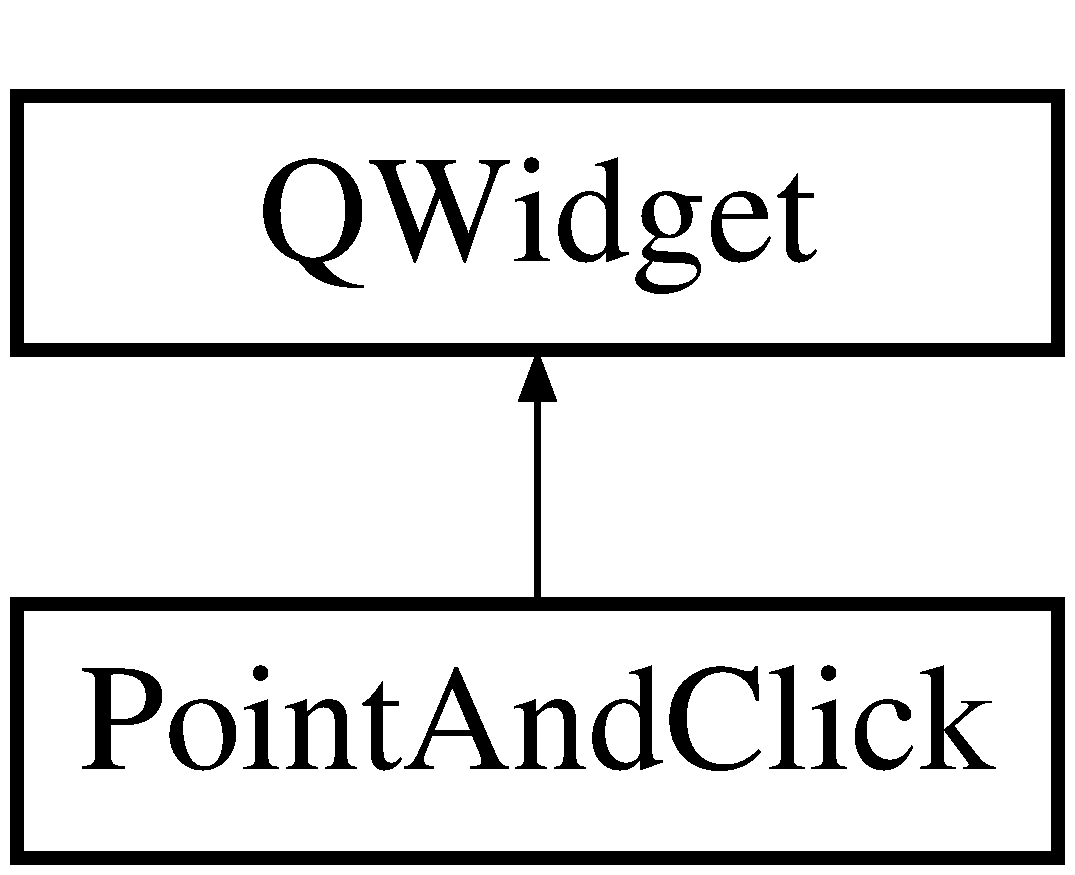
\includegraphics[height=2.000000cm]{class_point_and_click}
\end{center}
\end{figure}
\subsection*{Public Member Functions}
\begin{DoxyCompactItemize}
\item 
\mbox{\Hypertarget{class_point_and_click_a23e3974c812b2dd2c3e8da120e694aca}\label{class_point_and_click_a23e3974c812b2dd2c3e8da120e694aca}} 
\hyperlink{class_point_and_click_a23e3974c812b2dd2c3e8da120e694aca}{Point\+And\+Click} (Q\+Widget $\ast$parent=0)
\begin{DoxyCompactList}\small\item\em Constructeur et destructeur. \end{DoxyCompactList}\end{DoxyCompactItemize}


The documentation for this class was generated from the following files\+:\begin{DoxyCompactItemize}
\item 
C\+:/\+Users/\+Jean-\/\+Loup/\+Documents/\+L3/\+Projet\+Malette\+Jeux/\+Q\+T/\+L\+W\+Robin/\+Learn\+With\+Robin\+Main/pointandclick.\+h\item 
C\+:/\+Users/\+Jean-\/\+Loup/\+Documents/\+L3/\+Projet\+Malette\+Jeux/\+Q\+T/\+L\+W\+Robin/\+Learn\+With\+Robin\+Main/pointandclick.\+cpp\end{DoxyCompactItemize}

\hypertarget{class_puzzle}{}\section{Puzzle Class Reference}
\label{class_puzzle}\index{Puzzle@{Puzzle}}
Inheritance diagram for Puzzle\+:\begin{figure}[H]
\begin{center}
\leavevmode
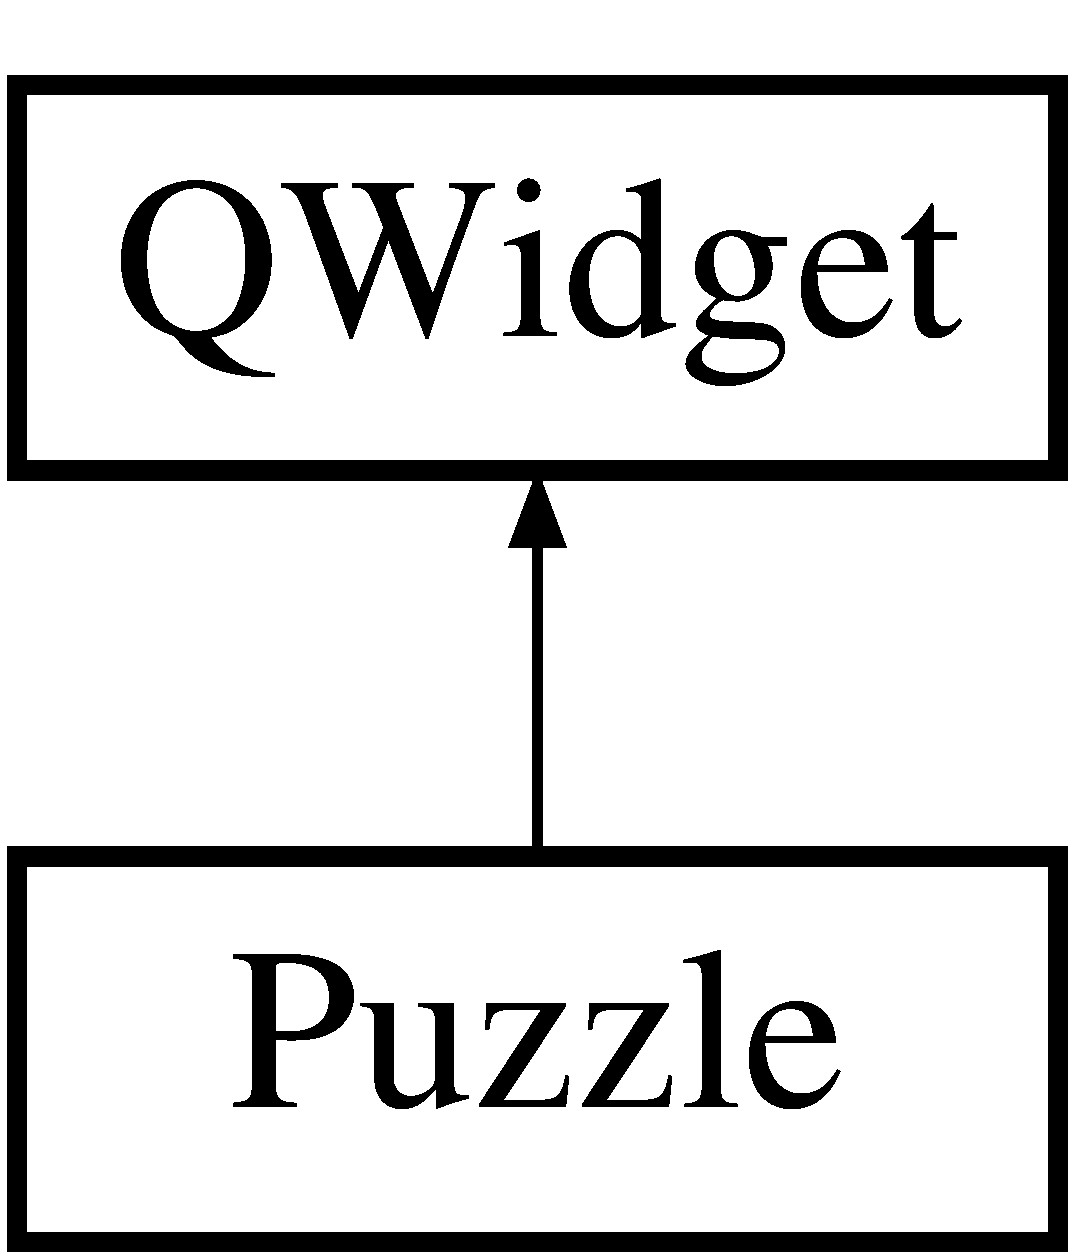
\includegraphics[height=2.000000cm]{class_puzzle}
\end{center}
\end{figure}
\subsection*{Public Member Functions}
\begin{DoxyCompactItemize}
\item 
\mbox{\Hypertarget{class_puzzle_a9781d5d1803efc344bc3d9c13f2451dc}\label{class_puzzle_a9781d5d1803efc344bc3d9c13f2451dc}} 
\hyperlink{class_puzzle_a9781d5d1803efc344bc3d9c13f2451dc}{Puzzle} (Q\+Widget $\ast$parent=0)
\begin{DoxyCompactList}\small\item\em Constructeur et destructeur. \end{DoxyCompactList}\end{DoxyCompactItemize}


The documentation for this class was generated from the following files\+:\begin{DoxyCompactItemize}
\item 
C\+:/\+Users/\+Jean-\/\+Loup/\+Documents/\+L3/\+Projet\+Malette\+Jeux/\+Q\+T/\+L\+W\+Robin/\+Learn\+With\+Robin\+Main/puzzle.\+h\item 
C\+:/\+Users/\+Jean-\/\+Loup/\+Documents/\+L3/\+Projet\+Malette\+Jeux/\+Q\+T/\+L\+W\+Robin/\+Learn\+With\+Robin\+Main/puzzle.\+cpp\end{DoxyCompactItemize}

\hypertarget{class_robin_main_window}{}\section{Robin\+Main\+Window Class Reference}
\label{class_robin_main_window}\index{Robin\+Main\+Window@{Robin\+Main\+Window}}
Inheritance diagram for Robin\+Main\+Window\+:\begin{figure}[H]
\begin{center}
\leavevmode
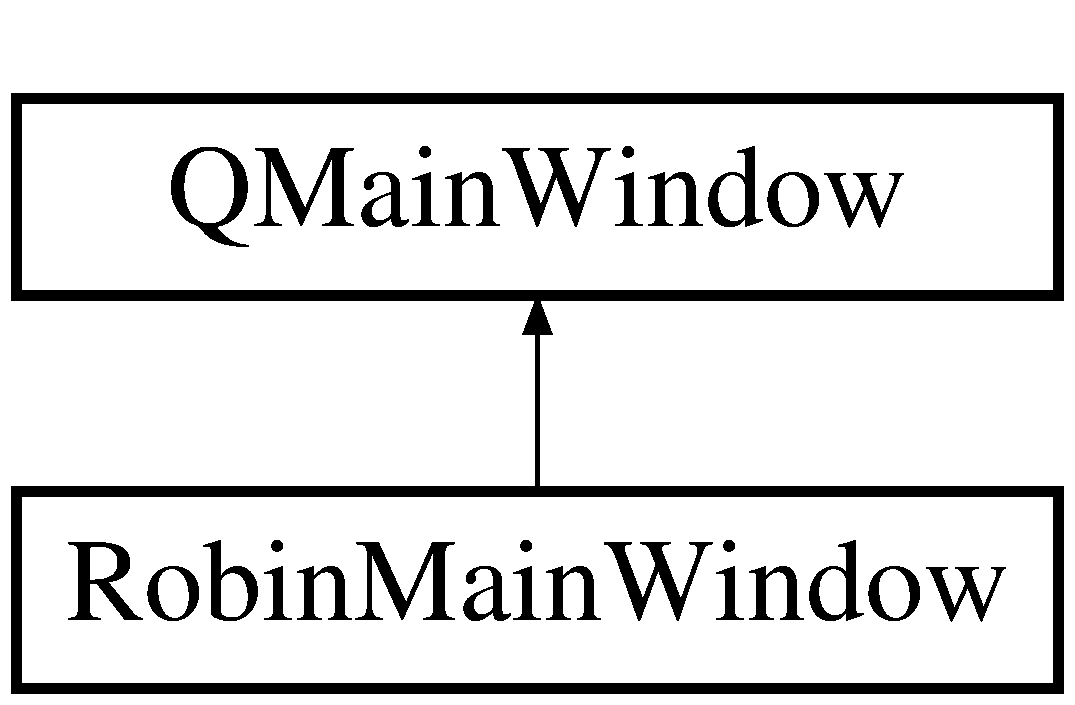
\includegraphics[height=2.000000cm]{class_robin_main_window}
\end{center}
\end{figure}
\subsection*{Public Slots}
\begin{DoxyCompactItemize}
\item 
void \hyperlink{class_robin_main_window_a08e1d2b660c03aa711d552258a368ec0}{game\+Ended} (std\+::pair$<$ std\+::string, int $>$ asso)
\begin{DoxyCompactList}\small\item\em Slot d\textquotesingle{}attente de fin de jeu. \end{DoxyCompactList}\item 
void \hyperlink{class_robin_main_window_a0850e17ae24394b14eb2dcfc4f15eeca}{back\+To\+Menu} (void)
\begin{DoxyCompactList}\small\item\em Signal pour retourner au menu principal. \end{DoxyCompactList}\item 
void \hyperlink{class_robin_main_window_a55e49d0a4d727066b553fc2277dd8a78}{open\+Calcul} (void)
\begin{DoxyCompactList}\small\item\em Signal pour lancer le calcul mental. \end{DoxyCompactList}\item 
void \hyperlink{class_robin_main_window_ab00b403de3169493a08c53f5d623ce6b}{open\+Simon} (void)
\begin{DoxyCompactList}\small\item\em Signal pour lancer le super simon. \end{DoxyCompactList}\item 
void \hyperlink{class_robin_main_window_aaf62641d678eb0f8829a2fb9c513ae68}{open\+Memory} (void)
\begin{DoxyCompactList}\small\item\em Signal pour lancer le memory. \end{DoxyCompactList}\item 
\mbox{\Hypertarget{class_robin_main_window_a3fb974c65b231fe737c9574acf989c36}\label{class_robin_main_window_a3fb974c65b231fe737c9574acf989c36}} 
void \hyperlink{class_robin_main_window_a3fb974c65b231fe737c9574acf989c36}{save\+Score\+Test} (void)
\begin{DoxyCompactList}\small\item\em Sauvegarde de score de test. \end{DoxyCompactList}\item 
\mbox{\Hypertarget{class_robin_main_window_a8bd52ec1bdbcbeaee45005ce4f0196f3}\label{class_robin_main_window_a8bd52ec1bdbcbeaee45005ce4f0196f3}} 
void \hyperlink{class_robin_main_window_a8bd52ec1bdbcbeaee45005ce4f0196f3}{change\+Player} (void)
\begin{DoxyCompactList}\small\item\em Changement de joueur. \end{DoxyCompactList}\end{DoxyCompactItemize}
\subsection*{Public Member Functions}
\begin{DoxyCompactItemize}
\item 
\hyperlink{class_robin_main_window_a55f7775f5daefb2099a51e97d50df666}{Robin\+Main\+Window} (Q\+Widget $\ast$parent=0)
\begin{DoxyCompactList}\small\item\em Constructeur et destructeur. \end{DoxyCompactList}\item 
\hyperlink{class_robin_main_window_a72eb8450efc1dfe22e2f36c7f728c5f3}{$\sim$\+Robin\+Main\+Window} ()
\item 
\mbox{\Hypertarget{class_robin_main_window_a66991c9057efd1d3ebc38e57e8df5b72}\label{class_robin_main_window_a66991c9057efd1d3ebc38e57e8df5b72}} 
void \hyperlink{class_robin_main_window_a66991c9057efd1d3ebc38e57e8df5b72}{set\+At\+Menu} (bool am)
\begin{DoxyCompactList}\small\item\em Getter setter. \end{DoxyCompactList}\item 
\mbox{\Hypertarget{class_robin_main_window_a8d360dc6f209df2b1567f8c787dd49c7}\label{class_robin_main_window_a8d360dc6f209df2b1567f8c787dd49c7}} 
bool {\bfseries get\+At\+Menu} (void)
\end{DoxyCompactItemize}


\subsection{Constructor \& Destructor Documentation}
\mbox{\Hypertarget{class_robin_main_window_a55f7775f5daefb2099a51e97d50df666}\label{class_robin_main_window_a55f7775f5daefb2099a51e97d50df666}} 
\index{Robin\+Main\+Window@{Robin\+Main\+Window}!Robin\+Main\+Window@{Robin\+Main\+Window}}
\index{Robin\+Main\+Window@{Robin\+Main\+Window}!Robin\+Main\+Window@{Robin\+Main\+Window}}
\subsubsection{\texorpdfstring{Robin\+Main\+Window()}{RobinMainWindow()}}
{\footnotesize\ttfamily Robin\+Main\+Window\+::\+Robin\+Main\+Window (\begin{DoxyParamCaption}\item[{Q\+Widget $\ast$}]{parent = {\ttfamily 0} }\end{DoxyParamCaption})\hspace{0.3cm}{\ttfamily [explicit]}}



Constructeur et destructeur. 

\hyperlink{class_robin_main_window_a55f7775f5daefb2099a51e97d50df666}{Robin\+Main\+Window\+::\+Robin\+Main\+Window} I\+N\+D\+EX des jeux dans le Q\+Stacked\+Widget d\textquotesingle{}affichage 0 M\+E\+NU 1 C\+A\+L\+C\+UL 2 S\+I\+M\+ON 3 M\+E\+M\+O\+RY 4 F\+L\+A\+GS 5 P\+U\+Z\+Z\+LE 6 P\+O\+I\+NT.

\begin{DoxyRefDesc}{Todo}
\item[\hyperlink{todo__todo000019}{Todo}]bien penser a connecter les boutons nécessaires quand on charge un widget quand le bouton menu sera passé dans chaque widget notamment \end{DoxyRefDesc}
\begin{DoxyRefDesc}{Test}
\item[\hyperlink{test__test000004}{Test}]changer la fenetre on peut tenter vu que Q\+Widget hérite de Q\+Object \end{DoxyRefDesc}


\begin{DoxyRefDesc}{Test}
\item[\hyperlink{test__test000005}{Test}]test très fort \end{DoxyRefDesc}


creation wid\+Stack

affichage du menu \mbox{\Hypertarget{class_robin_main_window_a72eb8450efc1dfe22e2f36c7f728c5f3}\label{class_robin_main_window_a72eb8450efc1dfe22e2f36c7f728c5f3}} 
\index{Robin\+Main\+Window@{Robin\+Main\+Window}!````~Robin\+Main\+Window@{$\sim$\+Robin\+Main\+Window}}
\index{````~Robin\+Main\+Window@{$\sim$\+Robin\+Main\+Window}!Robin\+Main\+Window@{Robin\+Main\+Window}}
\subsubsection{\texorpdfstring{$\sim$\+Robin\+Main\+Window()}{~RobinMainWindow()}}
{\footnotesize\ttfamily Robin\+Main\+Window\+::$\sim$\+Robin\+Main\+Window (\begin{DoxyParamCaption}{ }\end{DoxyParamCaption})}

\begin{DoxyRefDesc}{Todo}
\item[\hyperlink{todo__todo000020}{Todo}]faire une fonction qui vide le widget \end{DoxyRefDesc}


\subsection{Member Function Documentation}
\mbox{\Hypertarget{class_robin_main_window_a0850e17ae24394b14eb2dcfc4f15eeca}\label{class_robin_main_window_a0850e17ae24394b14eb2dcfc4f15eeca}} 
\index{Robin\+Main\+Window@{Robin\+Main\+Window}!back\+To\+Menu@{back\+To\+Menu}}
\index{back\+To\+Menu@{back\+To\+Menu}!Robin\+Main\+Window@{Robin\+Main\+Window}}
\subsubsection{\texorpdfstring{back\+To\+Menu}{backToMenu}}
{\footnotesize\ttfamily void Robin\+Main\+Window\+::back\+To\+Menu (\begin{DoxyParamCaption}\item[{void}]{ }\end{DoxyParamCaption})\hspace{0.3cm}{\ttfamily [slot]}}



Signal pour retourner au menu principal. 



 \subsubsection*{S\+L\+O\+TS }

\begin{DoxyRefDesc}{Todo}
\item[\hyperlink{todo__todo000021}{Todo}]bien penser a reconnecter tout \end{DoxyRefDesc}
\mbox{\Hypertarget{class_robin_main_window_a08e1d2b660c03aa711d552258a368ec0}\label{class_robin_main_window_a08e1d2b660c03aa711d552258a368ec0}} 
\index{Robin\+Main\+Window@{Robin\+Main\+Window}!game\+Ended@{game\+Ended}}
\index{game\+Ended@{game\+Ended}!Robin\+Main\+Window@{Robin\+Main\+Window}}
\subsubsection{\texorpdfstring{game\+Ended}{gameEnded}}
{\footnotesize\ttfamily void Robin\+Main\+Window\+::game\+Ended (\begin{DoxyParamCaption}\item[{std\+::pair$<$ std\+::string, int $>$}]{asso }\end{DoxyParamCaption})\hspace{0.3cm}{\ttfamily [slot]}}



Slot d\textquotesingle{}attente de fin de jeu. 

Fait apparaitre une popup de récapitulation \mbox{\Hypertarget{class_robin_main_window_a55e49d0a4d727066b553fc2277dd8a78}\label{class_robin_main_window_a55e49d0a4d727066b553fc2277dd8a78}} 
\index{Robin\+Main\+Window@{Robin\+Main\+Window}!open\+Calcul@{open\+Calcul}}
\index{open\+Calcul@{open\+Calcul}!Robin\+Main\+Window@{Robin\+Main\+Window}}
\subsubsection{\texorpdfstring{open\+Calcul}{openCalcul}}
{\footnotesize\ttfamily void Robin\+Main\+Window\+::open\+Calcul (\begin{DoxyParamCaption}\item[{void}]{ }\end{DoxyParamCaption})\hspace{0.3cm}{\ttfamily [slot]}}



Signal pour lancer le calcul mental. 

\begin{DoxyRefDesc}{Todo}
\item[\hyperlink{todo__todo000022}{Todo}]completer \end{DoxyRefDesc}
\mbox{\Hypertarget{class_robin_main_window_aaf62641d678eb0f8829a2fb9c513ae68}\label{class_robin_main_window_aaf62641d678eb0f8829a2fb9c513ae68}} 
\index{Robin\+Main\+Window@{Robin\+Main\+Window}!open\+Memory@{open\+Memory}}
\index{open\+Memory@{open\+Memory}!Robin\+Main\+Window@{Robin\+Main\+Window}}
\subsubsection{\texorpdfstring{open\+Memory}{openMemory}}
{\footnotesize\ttfamily void Robin\+Main\+Window\+::open\+Memory (\begin{DoxyParamCaption}\item[{void}]{ }\end{DoxyParamCaption})\hspace{0.3cm}{\ttfamily [slot]}}



Signal pour lancer le memory. 

\begin{DoxyRefDesc}{Todo}
\item[\hyperlink{todo__todo000024}{Todo}]completer \end{DoxyRefDesc}
\mbox{\Hypertarget{class_robin_main_window_ab00b403de3169493a08c53f5d623ce6b}\label{class_robin_main_window_ab00b403de3169493a08c53f5d623ce6b}} 
\index{Robin\+Main\+Window@{Robin\+Main\+Window}!open\+Simon@{open\+Simon}}
\index{open\+Simon@{open\+Simon}!Robin\+Main\+Window@{Robin\+Main\+Window}}
\subsubsection{\texorpdfstring{open\+Simon}{openSimon}}
{\footnotesize\ttfamily void Robin\+Main\+Window\+::open\+Simon (\begin{DoxyParamCaption}\item[{void}]{ }\end{DoxyParamCaption})\hspace{0.3cm}{\ttfamily [slot]}}



Signal pour lancer le super simon. 

\begin{DoxyRefDesc}{Todo}
\item[\hyperlink{todo__todo000023}{Todo}]completer \end{DoxyRefDesc}


The documentation for this class was generated from the following files\+:\begin{DoxyCompactItemize}
\item 
C\+:/\+Users/\+Jean-\/\+Loup/\+Documents/\+L3/\+Projet\+Malette\+Jeux/\+Q\+T/\+L\+W\+Robin/\+Learn\+With\+Robin\+Main/robinmainwindow.\+h\item 
C\+:/\+Users/\+Jean-\/\+Loup/\+Documents/\+L3/\+Projet\+Malette\+Jeux/\+Q\+T/\+L\+W\+Robin/\+Learn\+With\+Robin\+Main/robinmainwindow.\+cpp\end{DoxyCompactItemize}

\hypertarget{class_super_simon}{}\section{Super\+Simon Class Reference}
\label{class_super_simon}\index{Super\+Simon@{Super\+Simon}}
Inheritance diagram for Super\+Simon\+:\begin{figure}[H]
\begin{center}
\leavevmode
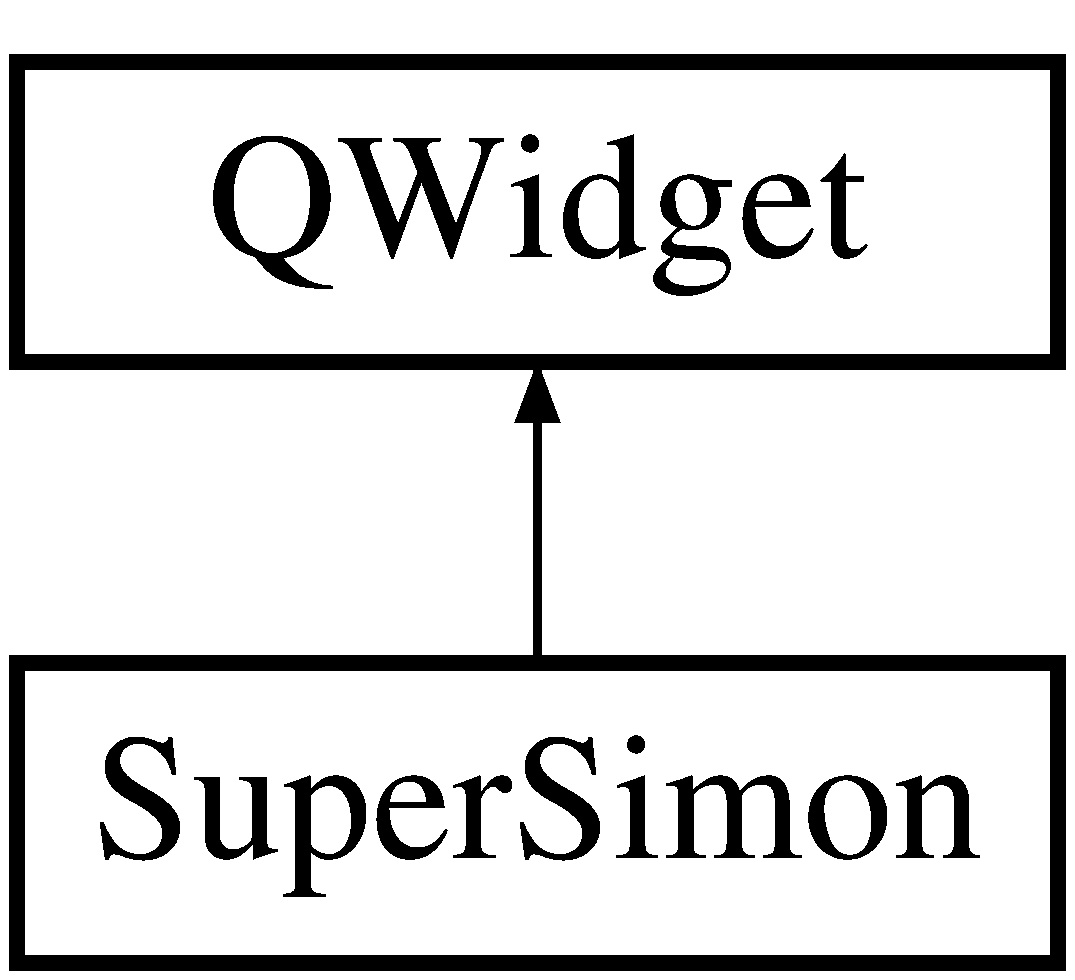
\includegraphics[height=2.000000cm]{class_super_simon}
\end{center}
\end{figure}
\subsection*{Public Slots}
\begin{DoxyCompactItemize}
\item 
void \hyperlink{class_super_simon_af495f2a329d2966c2f265cb46753a13d}{simon\+Clicked\+Redirect} ()
\begin{DoxyCompactList}\small\item\em Appui sur bouton du simon. \end{DoxyCompactList}\item 
\mbox{\Hypertarget{class_super_simon_accceee26094ef9d22fe8b3934f34e607}\label{class_super_simon_accceee26094ef9d22fe8b3934f34e607}} 
void \hyperlink{class_super_simon_accceee26094ef9d22fe8b3934f34e607}{simon\+Clicked} (const int)
\begin{DoxyCompactList}\small\item\em Appui sur bouton du simon. \end{DoxyCompactList}\item 
\mbox{\Hypertarget{class_super_simon_a5a68e15b3f3322e083dc89dc6379cc91}\label{class_super_simon_a5a68e15b3f3322e083dc89dc6379cc91}} 
void \hyperlink{class_super_simon_a5a68e15b3f3322e083dc89dc6379cc91}{add\+Life\+Clicked} ()
\begin{DoxyCompactList}\small\item\em Redirection vers life\+Clicked avec la valeur du bouton. \end{DoxyCompactList}\item 
\mbox{\Hypertarget{class_super_simon_a56553d0c5ff5bfa19ef7a6b6bbbac672}\label{class_super_simon_a56553d0c5ff5bfa19ef7a6b6bbbac672}} 
void \hyperlink{class_super_simon_a56553d0c5ff5bfa19ef7a6b6bbbac672}{rem\+Life\+Clicked} ()
\begin{DoxyCompactList}\small\item\em Appui sur un modificateur de vie. \end{DoxyCompactList}\item 
\mbox{\Hypertarget{class_super_simon_aa0b9fa2f2d980039b2cc3b5e5f98c51f}\label{class_super_simon_aa0b9fa2f2d980039b2cc3b5e5f98c51f}} 
void \hyperlink{class_super_simon_aa0b9fa2f2d980039b2cc3b5e5f98c51f}{read\+Sequence\+Clicked} (void)
\begin{DoxyCompactList}\small\item\em Appui sur read sequence. \end{DoxyCompactList}\item 
\mbox{\Hypertarget{class_super_simon_a4dd6e368e1dca177272e937209ff4974}\label{class_super_simon_a4dd6e368e1dca177272e937209ff4974}} 
void \hyperlink{class_super_simon_a4dd6e368e1dca177272e937209ff4974}{edit\+Sequence\+Clicked} (void)
\begin{DoxyCompactList}\small\item\em Appui sur edit sequence. \end{DoxyCompactList}\item 
void \hyperlink{class_super_simon_a81bff9afba77880d36563aac5534ccd3}{reset\+Score\+Clicked} (void)
\begin{DoxyCompactList}\small\item\em Appui sur reset score. \end{DoxyCompactList}\item 
\mbox{\Hypertarget{class_super_simon_aa8c1d5cee800c30c2eda3d4e32a438eb}\label{class_super_simon_aa8c1d5cee800c30c2eda3d4e32a438eb}} 
void \hyperlink{class_super_simon_aa8c1d5cee800c30c2eda3d4e32a438eb}{delete\+Audio} (void)
\begin{DoxyCompactList}\small\item\em Supprime les éléments responsables du son. \end{DoxyCompactList}\end{DoxyCompactItemize}
\subsection*{Signals}
\begin{DoxyCompactItemize}
\item 
\mbox{\Hypertarget{class_super_simon_ac03f5803072330be308372659c5ffb1c}\label{class_super_simon_ac03f5803072330be308372659c5ffb1c}} 
void \hyperlink{class_super_simon_ac03f5803072330be308372659c5ffb1c}{end\+Of\+Game} (std\+::pair$<$ std\+::string, int $>$ asso)
\begin{DoxyCompactList}\small\item\em fin du jeu \end{DoxyCompactList}\end{DoxyCompactItemize}
\subsection*{Public Member Functions}
\begin{DoxyCompactItemize}
\item 
\hyperlink{class_super_simon_a203f799a56234b59ba692ed5b7a74537}{Super\+Simon} (Q\+Widget $\ast$parent=nullptr)
\begin{DoxyCompactList}\small\item\em Constructeur destructeur. \end{DoxyCompactList}\item 
\mbox{\Hypertarget{class_super_simon_a1676872fe3b03afef6ce057beae773b8}\label{class_super_simon_a1676872fe3b03afef6ce057beae773b8}} 
void \hyperlink{class_super_simon_a1676872fe3b03afef6ce057beae773b8}{read\+Sequence} (void)
\begin{DoxyCompactList}\small\item\em Lire la séquence actuelle (joue et affiche en toutes lettres le nom des couleurs) \end{DoxyCompactList}\item 
void \hyperlink{class_super_simon_af00408823847e80a511019baa536afb3}{edit\+Sequence} (void)
\begin{DoxyCompactList}\small\item\em Editer la séquence à jouer. \end{DoxyCompactList}\item 
\mbox{\Hypertarget{class_super_simon_a611cecfe4b8945c9ce70c206e64a6038}\label{class_super_simon_a611cecfe4b8945c9ce70c206e64a6038}} 
void \hyperlink{class_super_simon_a611cecfe4b8945c9ce70c206e64a6038}{add\+Life} (void)
\begin{DoxyCompactList}\small\item\em Ajouter une vie au joueur. \end{DoxyCompactList}\item 
\mbox{\Hypertarget{class_super_simon_a081108169be3715de506ccaebebf01d9}\label{class_super_simon_a081108169be3715de506ccaebebf01d9}} 
void \hyperlink{class_super_simon_a081108169be3715de506ccaebebf01d9}{rem\+Life} (void)
\begin{DoxyCompactList}\small\item\em Retirer une vie au joueur. \end{DoxyCompactList}\item 
\mbox{\Hypertarget{class_super_simon_a9c3cccc53f6445c0bf03b30dd6528340}\label{class_super_simon_a9c3cccc53f6445c0bf03b30dd6528340}} 
void \hyperlink{class_super_simon_a9c3cccc53f6445c0bf03b30dd6528340}{res\+Score} (void)
\begin{DoxyCompactList}\small\item\em Réinitialiser le score. \end{DoxyCompactList}\item 
void \hyperlink{class_super_simon_aece1587ad880233a11cf24cbbe284a42}{add\+To\+Sequence} (int)
\begin{DoxyCompactList}\small\item\em Ajoute l\textquotesingle{}entier représentant un bouton au Q\+String seq\+Entered. \end{DoxyCompactList}\item 
void \hyperlink{class_super_simon_a4ea2f32b57775bd2c784472369127bcf}{check\+Seq\+Lenght} (void)
\begin{DoxyCompactList}\small\item\em Vérifie la taille de seq\+Entered. \end{DoxyCompactList}\item 
\mbox{\Hypertarget{class_super_simon_a242ac18e5bcd7487bfd8a5b01b59669a}\label{class_super_simon_a242ac18e5bcd7487bfd8a5b01b59669a}} 
bool \hyperlink{class_super_simon_a242ac18e5bcd7487bfd8a5b01b59669a}{send\+Seq\+For\+Check} (void)
\begin{DoxyCompactList}\small\item\em Envoie la séquence au modèle pour vérification. \end{DoxyCompactList}\item 
void \hyperlink{class_super_simon_a8d5c23562cd6b048720003d3c796ac7a}{update\+View\+Simon} (void)
\begin{DoxyCompactList}\small\item\em Mettre à jour la vue. \end{DoxyCompactList}\item 
void \hyperlink{class_super_simon_af12663f8a26a971a508a40a33d0afceb}{delay} (int \&sec)
\begin{DoxyCompactList}\small\item\em Attend sec secondes. \end{DoxyCompactList}\item 
\mbox{\Hypertarget{class_super_simon_ad579e5ed8007a599d5074299c4bee712}\label{class_super_simon_ad579e5ed8007a599d5074299c4bee712}} 
void \hyperlink{class_super_simon_ad579e5ed8007a599d5074299c4bee712}{send\+End\+Of\+Game} (void)
\begin{DoxyCompactList}\small\item\em Declencher fin du jeu. \end{DoxyCompactList}\item 
\mbox{\Hypertarget{class_super_simon_a3834147e3d6956d918a9ef31c4a87c3d}\label{class_super_simon_a3834147e3d6956d918a9ef31c4a87c3d}} 
bool \hyperlink{class_super_simon_a3834147e3d6956d918a9ef31c4a87c3d}{check\+End\+Of\+Game} (void)
\begin{DoxyCompactList}\small\item\em Verifier si fin du jeu. \end{DoxyCompactList}\end{DoxyCompactItemize}


\subsection{Constructor \& Destructor Documentation}
\mbox{\Hypertarget{class_super_simon_a203f799a56234b59ba692ed5b7a74537}\label{class_super_simon_a203f799a56234b59ba692ed5b7a74537}} 
\index{Super\+Simon@{Super\+Simon}!Super\+Simon@{Super\+Simon}}
\index{Super\+Simon@{Super\+Simon}!Super\+Simon@{Super\+Simon}}
\subsubsection{\texorpdfstring{Super\+Simon()}{SuperSimon()}}
{\footnotesize\ttfamily Super\+Simon\+::\+Super\+Simon (\begin{DoxyParamCaption}\item[{Q\+Widget $\ast$}]{parent = {\ttfamily nullptr} }\end{DoxyParamCaption})\hspace{0.3cm}{\ttfamily [explicit]}}



Constructeur destructeur. 

Pour info 1 \+: blue 2 \+: green 3 \+: red 4 \+: yellow

\subsection{Member Function Documentation}
\mbox{\Hypertarget{class_super_simon_aece1587ad880233a11cf24cbbe284a42}\label{class_super_simon_aece1587ad880233a11cf24cbbe284a42}} 
\index{Super\+Simon@{Super\+Simon}!add\+To\+Sequence@{add\+To\+Sequence}}
\index{add\+To\+Sequence@{add\+To\+Sequence}!Super\+Simon@{Super\+Simon}}
\subsubsection{\texorpdfstring{add\+To\+Sequence()}{addToSequence()}}
{\footnotesize\ttfamily void Super\+Simon\+::add\+To\+Sequence (\begin{DoxyParamCaption}\item[{int}]{num\+To\+Add }\end{DoxyParamCaption})}



Ajoute l\textquotesingle{}entier représentant un bouton au Q\+String seq\+Entered. 

Appelle check\+Seq\+Lenght \mbox{\Hypertarget{class_super_simon_a4ea2f32b57775bd2c784472369127bcf}\label{class_super_simon_a4ea2f32b57775bd2c784472369127bcf}} 
\index{Super\+Simon@{Super\+Simon}!check\+Seq\+Lenght@{check\+Seq\+Lenght}}
\index{check\+Seq\+Lenght@{check\+Seq\+Lenght}!Super\+Simon@{Super\+Simon}}
\subsubsection{\texorpdfstring{check\+Seq\+Lenght()}{checkSeqLenght()}}
{\footnotesize\ttfamily void Super\+Simon\+::check\+Seq\+Lenght (\begin{DoxyParamCaption}\item[{void}]{ }\end{DoxyParamCaption})}



Vérifie la taille de seq\+Entered. 

Appelle send\+Seq\+For\+Check si la taille attendue est atteinte \mbox{\Hypertarget{class_super_simon_af12663f8a26a971a508a40a33d0afceb}\label{class_super_simon_af12663f8a26a971a508a40a33d0afceb}} 
\index{Super\+Simon@{Super\+Simon}!delay@{delay}}
\index{delay@{delay}!Super\+Simon@{Super\+Simon}}
\subsubsection{\texorpdfstring{delay()}{delay()}}
{\footnotesize\ttfamily void Super\+Simon\+::delay (\begin{DoxyParamCaption}\item[{int \&}]{sec }\end{DoxyParamCaption})}



Attend sec secondes. 

\begin{DoxyRefDesc}{Test}
\item[\hyperlink{test__test000006}{Test}]\end{DoxyRefDesc}
\mbox{\Hypertarget{class_super_simon_af00408823847e80a511019baa536afb3}\label{class_super_simon_af00408823847e80a511019baa536afb3}} 
\index{Super\+Simon@{Super\+Simon}!edit\+Sequence@{edit\+Sequence}}
\index{edit\+Sequence@{edit\+Sequence}!Super\+Simon@{Super\+Simon}}
\subsubsection{\texorpdfstring{edit\+Sequence()}{editSequence()}}
{\footnotesize\ttfamily void Super\+Simon\+::edit\+Sequence (\begin{DoxyParamCaption}\item[{void}]{ }\end{DoxyParamCaption})}



Editer la séquence à jouer. 

\mbox{\Hypertarget{class_super_simon_a81bff9afba77880d36563aac5534ccd3}\label{class_super_simon_a81bff9afba77880d36563aac5534ccd3}} 
\index{Super\+Simon@{Super\+Simon}!reset\+Score\+Clicked@{reset\+Score\+Clicked}}
\index{reset\+Score\+Clicked@{reset\+Score\+Clicked}!Super\+Simon@{Super\+Simon}}
\subsubsection{\texorpdfstring{reset\+Score\+Clicked}{resetScoreClicked}}
{\footnotesize\ttfamily void Super\+Simon\+::reset\+Score\+Clicked (\begin{DoxyParamCaption}\item[{void}]{ }\end{DoxyParamCaption})\hspace{0.3cm}{\ttfamily [slot]}}



Appui sur reset score. 



 \subsubsection*{S\+L\+O\+TS }\mbox{\Hypertarget{class_super_simon_af495f2a329d2966c2f265cb46753a13d}\label{class_super_simon_af495f2a329d2966c2f265cb46753a13d}} 
\index{Super\+Simon@{Super\+Simon}!simon\+Clicked\+Redirect@{simon\+Clicked\+Redirect}}
\index{simon\+Clicked\+Redirect@{simon\+Clicked\+Redirect}!Super\+Simon@{Super\+Simon}}
\subsubsection{\texorpdfstring{simon\+Clicked\+Redirect}{simonClickedRedirect}}
{\footnotesize\ttfamily void Super\+Simon\+::simon\+Clicked\+Redirect (\begin{DoxyParamCaption}{ }\end{DoxyParamCaption})\hspace{0.3cm}{\ttfamily [slot]}}



Appui sur bouton du simon. 

Redirection vers simon\+Clicked avec la valeur du bouton \mbox{\Hypertarget{class_super_simon_a8d5c23562cd6b048720003d3c796ac7a}\label{class_super_simon_a8d5c23562cd6b048720003d3c796ac7a}} 
\index{Super\+Simon@{Super\+Simon}!update\+View\+Simon@{update\+View\+Simon}}
\index{update\+View\+Simon@{update\+View\+Simon}!Super\+Simon@{Super\+Simon}}
\subsubsection{\texorpdfstring{update\+View\+Simon()}{updateViewSimon()}}
{\footnotesize\ttfamily void Super\+Simon\+::update\+View\+Simon (\begin{DoxyParamCaption}\item[{void}]{ }\end{DoxyParamCaption})}



Mettre à jour la vue. 

\begin{DoxyRefDesc}{Todo}
\item[\hyperlink{todo__todo000025}{Todo}]mettre a jour les textes \end{DoxyRefDesc}


The documentation for this class was generated from the following files\+:\begin{DoxyCompactItemize}
\item 
C\+:/\+Users/\+Jean-\/\+Loup/\+Documents/\+L3/\+Projet\+Malette\+Jeux/\+Q\+T/\+L\+W\+Robin/\+Learn\+With\+Robin\+Main/supersimon.\+h\item 
C\+:/\+Users/\+Jean-\/\+Loup/\+Documents/\+L3/\+Projet\+Malette\+Jeux/\+Q\+T/\+L\+W\+Robin/\+Learn\+With\+Robin\+Main/supersimon.\+cpp\end{DoxyCompactItemize}

\hypertarget{class_tools}{}\section{Tools Class Reference}
\label{class_tools}\index{Tools@{Tools}}
\subsection*{Static Public Member Functions}
\begin{DoxyCompactItemize}
\item 
static void \hyperlink{class_tools_a5de09268ac074b96c2275ccad05316ca}{Save\+Player\+Score\+For\+Game} (std\+::string player, int score, std\+::string game)
\begin{DoxyCompactList}\small\item\em Enregistrer le score d\textquotesingle{}un joueur. \end{DoxyCompactList}\end{DoxyCompactItemize}


\subsection{Member Function Documentation}
\mbox{\Hypertarget{class_tools_a5de09268ac074b96c2275ccad05316ca}\label{class_tools_a5de09268ac074b96c2275ccad05316ca}} 
\index{Tools@{Tools}!Save\+Player\+Score\+For\+Game@{Save\+Player\+Score\+For\+Game}}
\index{Save\+Player\+Score\+For\+Game@{Save\+Player\+Score\+For\+Game}!Tools@{Tools}}
\subsubsection{\texorpdfstring{Save\+Player\+Score\+For\+Game()}{SavePlayerScoreForGame()}}
{\footnotesize\ttfamily void Tools\+::\+Save\+Player\+Score\+For\+Game (\begin{DoxyParamCaption}\item[{std\+::string}]{player,  }\item[{int}]{score,  }\item[{std\+::string}]{game }\end{DoxyParamCaption})\hspace{0.3cm}{\ttfamily [static]}}



Enregistrer le score d\textquotesingle{}un joueur. 


\begin{DoxyParams}{Parameters}
{\em player} & nom du joueur \\
\hline
{\em score} & score pour le jeu \\
\hline
{\em game} & jeu en question \\
\hline
\end{DoxyParams}


The documentation for this class was generated from the following files\+:\begin{DoxyCompactItemize}
\item 
C\+:/\+Users/\+Jean-\/\+Loup/\+Documents/\+L3/\+Projet\+Malette\+Jeux/\+Q\+T/\+L\+W\+Robin/\+Learn\+With\+Robin\+Main/tools.\+h\item 
C\+:/\+Users/\+Jean-\/\+Loup/\+Documents/\+L3/\+Projet\+Malette\+Jeux/\+Q\+T/\+L\+W\+Robin/\+Learn\+With\+Robin\+Main/tools.\+cpp\end{DoxyCompactItemize}

%--- End generated contents ---

% Index
\backmatter
\newpage
\phantomsection
\clearemptydoublepage
\addcontentsline{toc}{chapter}{Index}
\printindex

\end{document}
